\documentclass[sigconf, review, 10pt]{acmart} %timestamp 
%, timestamp
%\usepackage{usenix}
%end of changed lines
%\usepackage{microtype}
%\usepackage[hyphens]{url} %Option clash
\usepackage{balance}
\usepackage{leading}
\usepackage{graphicx}
\usepackage{subfig}
%Removing the geometry package used for Tighter Format
%\usepackage{geometry}
%\usepackage{times}
\usepackage{textcomp}
\usepackage{multirow}
\usepackage{framed}
\usepackage{amsmath}
\usepackage{listings}

\usepackage{enumitem}

%\usepackage[usenames,dvipsnames,svgnames,table]{xcolor} %Option Clash
%\usepackage[lined,noend,linesnumbered]{algorithm2e}
\usepackage{cleveref}

\crefformat{section}{\S#2#1#3} % see manual of cleveref, section 8.2.1

\newcommand{\sysname}{SciSpot\xspace}

%\newcommand{\comment}[1]{{\color{blue}[\textsf{#1}]}}

%\newcommand{\TODO}[1]{\comment{TODO: #1}}
%\renewcommand{\paragraph}[1]{\textbf{#1}}


\RequirePackage[normalem]{ulem}
\RequirePackage{color}\definecolor{RED}{rgb}{1,0,0}\definecolor{BLUE}{rgb}{0,0,1}
\providecommand{\DIFadd}[1]{{\protect\color{blue}\uwave{#1}}}
\providecommand{\DIFdel}[1]{{\protect\color{red}\sout{#1}}}
%DIF SAFE PREAMBLE
\providecommand{\DIFaddbegin}{}
\providecommand{\DIFaddend}{}
\providecommand{\DIFdelbegin}{}
\providecommand{\DIFdelend}{}
%DIF FLOATSAFE PREAMBLE
\providecommand{\DIFaddFL}[1]{\DIFadd{#1}}
\providecommand{\DIFdelFL}[1]{\DIFdel{#1}}
\providecommand{\DIFaddbeginFL}{}
\providecommand{\DIFaddendFL}{}
\providecommand{\DIFdelbeginFL}{}
\providecommand{\DIFdelendFL}{}
%DIF END PREAMBLE EXTENSION ADDED BY LATEXDIFF

\def\Section {\S}

\newcommand{\squishlist}{
 \begin{list}{$\bullet$}
  { \setlength{\itemsep}{0pt}
     \setlength{\parsep}{3pt}
     \setlength{\topsep}{3pt}
     \setlength{\partopsep}{0pt}
     \setlength{\leftmargin}{1.5em}
     \setlength{\labelwidth}{1em}
     \setlength{\labelsep}{0.5em} } }
	
\newcommand{\squishlisttwo}{
 \begin{list}{$\bullet$}
  { \setlength{\itemsep}{0pt}
     \setlength{\parsep}{0pt}
    \setlength{\topsep}{0pt}
    \setlength{\partopsep}{0pt}
    \setlength{\leftmargin}{2em}
    \setlength{\labelwidth}{1.5em}
    \setlength{\labelsep}{0.5em} } }

\newcommand{\squishend}{
  \end{list}  }

\newcommand{\alert}[1] {\textcolor{red} {\textsc{#1}}}

\newcommand{\myfbox}[1] {\noindent \fbox{\parbox{0.5\textwidth} {#1}}}

\newcommand{\mhead}[1] {\noindent \textbf{#1}}

\newcommand*\mean[1]{\overline{#1}}

\newcommand{\eat}[1]{}

\newcommand{\compresslist}{%
  \setlength{\itemsep}{1pt}%
  \setlength{\leftmargin}{1.5em}
  \setlength{\labelwidth}{1em}
  \setlength{\parskip}{0pt}%
  \setlength{\parsep}{0pt}%
%  \setlength{\itemindent}{-10pt}%
}

\newcommand{\myfigspace}[0]{-0.45cm}
\newcommand{\bigfigspace}[0]{-0.9cm}
\newcommand{\captionspace}[0]{-0.5cm}
\newcommand{\subsecspace}[0]{-0.33cm}
\newcommand{\largesubsecspace}[0]{-0.40cm}
\newcommand{\tightext}[0]{-0.12cm}
\newcommand{\eqnspace}[0]{-0.1cm}

%%% Local Variables:
%%% mode: latex
%%% TeX-master: "paper"
%%% End:


\newcommand{\sign}[1]{\operatorname{sign}\left({#1}\right)}


\newcommand\prat[1]{\textcolor{red}{(Prateek: #1)}}
\newcommand\vikram[1]{\textcolor{green}{(Vikram: #1)}}


%%%%%%%% For submission only

\setcopyright{none}
\settopmatter{printacmref=false}
\acmConference{}{}{}
\acmPrice{}
\acmISBN{}
\acmDOI{}
\acmYear{}
\acmMonth{}
\settopmatter{printfolios=true}
%%%%%%%%%%%%%%%%%%%


\begin{document}
\title{SciSpot}
\author{Paper \# XXX}{}{}

\begin{abstract}
  In this paper, we...
%%% Local Variables:
%%% mode: latex
%%% TeX-master: "paper"
%%% End:

\end{abstract}

\maketitle

\section{Introduction}

Running parallel scientific applications, such as molecular dynamics (MD) simulations, on low-cost cloud transient resources. 

The first "big" idea is that simulations are often bag of parallel tasks. 

While there has been some past work that looks at running MPI applications on spot instances, our scope is much broader and considers how complete simulation pipelines can be run at low cost. 

Spiel on transient instances. Increasingly popular resource allocation model that is being offered by all cloud providers. 
Very low cost compared to conventional cloud resources, often by up to 10x. 
However, can be frequently revoked. 
Thus failure is a common occurrence, and not a rare-event. 
This is especially challenging for MPI jobs because of its inability to tolerate failures. 

However, our insight is that while protecting a *single* job against revocations can require elaborate checkpointing based approaches, we dont necessarily have to do that if we consider that most simulations are composed of a series of jobs that search over a parameter space, and that what is important is the total running time and cost of this entire series of jobs. 

Thus, no single job is "special". 

Another aspect of novelty is that past work on transient resources used EC2 pricing information to get failure probabilities. However, this is no longer an accurate method. We perform the first empirical study of google preemptible VMs and their performance and availability for HPC workloads. 

Another fundamental question is what is a suitable metric in such cases. Conventionally, it is speedup. In the cloud, it is some combination of cost and running time. 

%%% Local Variables:
%%% mode: latex
%%% TeX-master: "paper"
%%% End:


\sysname is a framework and a tool that combines the use of failure modeling, checkpointing, and application-aware early stopping, to provide low cost execution of jobgroups for scientific applications.


Our work is the first to make a principled study of transient instances \emph{other} than Amazon spot instances.
Furthermore, our techniques make the first stab at addressing the new problems in the new EC2 spot pricing scheme.





\section{Background}

\subsection{Transient Computing}

%\subsection{Heterogeneity and Parallel Scientific Applications in the Cloud}

%No extra parallelism required
%RM heterogen

%
\subsection{Case Studies: Bags of Jobs in Scientific Computing Applications}

\begin{comment}
Describe the kind of computation. DONE

Scaling properties. Almost perfectly scalable with O(n) communication? UNCLEAR WHAT IS MEANT TO BE DONE HERE

This can be a like a case study of parallel scientific simulations.
Will help relate to parameters etc with more concrete examples. DONE

Bag of jobs.
Why multiple runs: parameter sweeps, search, or just multiple times to get confidence intervals and stable results in case of randomness. 
DONE I THINK
\end{comment}

For testing and evaluating the SciSpot framework, we consider three representative examples (case studies) from molecular dynamics (MD) and hydrodynamics simulations: 1) MD simulations of ions in nanoscale confinement created by material surfaces \cite{jjzo1,kadupitiya2017}, MD-based optimization dynamics of shape-changing deformable nanoparticles (NPs) \cite{jto1,jyto}, and hydrodynamics simulations of continuum material models using the Livermore Unstructured Lagrangian Explicit Shock Hydrodynamics (LULESH) code \cite{IPDPS13:LULESH,LULESH2:changes}. These examples are representative of typical scientific computing applications in the broad domain of physics, materials science, and chemical engineering; the first two applications (1 and 2) are based on codes and associated theoretical formulations developed by us \cite{jso1,jso2,solis2013generating,jjzo1,jto1,jyto}, and case study 3 is based on an open-source code developed at Lawrence Livermore National Laboratories \cite{IPDPS13:LULESH,LULESH:spec}. These three examples are implemented as parallel programs that use OpenMP and MPI parallel computing techniques.

The typical workflow associated with most scientific computing applications, including the aforementioned case studies, involves the implementation of the ``bags of jobs'' approach at many critical stages. In the initial stage, the construction and calibration of the appropriate model often involves testing for the needed attributes (e.g., characteristic sizes, interactions potentials) of the building blocks (model components) by sweeping over different combinations of physical as well as computing parameters (e.g., simulation timestep, thermostat variables) and eliminating the sets that lead to unphysical, unstable, or computationally intractable scenarios. During the model examination stage for the investigation of the accuracy and generalization of the model to describe the associated natural or synthetic processes, the dynamics of the model system is simulated over a wide range of model parameters. Accordingly, multiple sets of simulations (bags of jobs) are run to sweep over a broad region of the multidimensional parameter space and to isolate the domains where the model works best and where it yields a poorer representation of the real system. 

Often, the key objective of the scientific computing application is to isolate the model system parameters where interesting changes in the material structure or assembly behaviors (e.g., phase transitions) are observed. A similar bags of jobs approach is also  adopted in such applications with the search for these model parameters generally inspired by experimentally-informed observations and/or predictions yielding from approximate analytical theoretical formulations. For example, in the simulation of deformable nanoparticles implemented in the NP shape code, one is interested in isolating the set of NP and environmental parameters: NP bending modulus, NP stretching constant, NP charge, and salt concentration, that yields complex NP deformations/shapes (e.g., discs, rods, bowls). Similarly, in the ions in nanoconfinement application, a quantity of interest is the set of electrolyte system attributes (parameters): confinement length $h$, positive ion valency ($z_p$), negative ion valency ($z_n$), electrolyte concentration $c$, and ion diameter $d$, that yields the expected contact density or the experimentally-measured effective pressure between the confining nanomaterial surfaces. Finally, the bags of jobs approach is adopted during the completion process in the workflow where simulations are often launched in parallel to fill any gaps in the extracted trends or to obtain error bars on the predictions (e.g., ionic density profiles, energy distributions, NP shape transitions).

In addition to the conventional scientific computing (HPC) applications, an emerging area of research in a broad range of fields including materials science, biology, neuroscience, and physics where the bags of jobs approach is critical to the workflow is the integration of machine learning (ML) tools with these HPC applications  \citep{ml.atomic2017,melko2017,sam2017,fu2017,long2015machine, ferguson2017machine,ward2018matminer,jcs1,jcs2,fox2019learning}. ML methods have been developed and implemented to identify model attributes/parameters that yield desirable material configurations \citep{glotzer2017}, update configurations in simulations \citep{botu2015adaptive,fu2017}, predict and auto-tune optimal simulation control parameters \cite{jcs1}, predict critical features associated with simulation output \cite{jcs2}, infer assembly landscapes \citep{long2015machine,ferguson2017machine}, and classify phases of matter \citep{melko2017}. In many of these examples, ML models (e.g., artificial neural network, support vector machines) are trained on large data sets generated via simulations run over a broad range of parameter values. The bags of jobs process is invoked multiple times during the experimentation with many ML techniques using training and testing datasets to isolate the ML method(s) that yield the most accurate results for a given scientific computing application. For example, in Ref.~\cite{jcs2}, an ANN was trained to predict contact, peak, and mid-point ionic density using training and testing datasets comprising of $\approx4800$ and $\approx2000$ simulation runs respectively. Datasets were generated using HPC resources (Bigred2 computing cluster) based on the sweep of parameters $h \in (3.0, 4.0)$ nm,  $z_p \in 1,2,3$ (in units of electronic charge $|e|$); $z_n \in -1,-2$ $|e|$; $c \in (0.3,0.9)$ M, and $d \in (0.5,0.75)$ nm. We envision the SciSpot framework described here to complement and supplement conventional HPC supercomputer systems in enabling the construction of such ML layers (wrappers) \cite{jcs2,fox2019learning} around scientific computing applications. 

%%% Local Variables:
%%% mode: latex
%%% TeX-master: "paper"
%%% End:


%\section{Understanding and Modeling Transient Server Preemptions}
%\section{Modeling the Dynamics of Transient Server Preemptions}
%\section{Preemption Dynamics of Transient Cloud Servers}
\vspace*{\subsecspace}
\section{Constrained Preemptions of Google Preemptible VMs}
\label{sec:failmodel}

%Understanding the nature and dynamics of transient cloud servers such as their preemption frequency is a prerequisite to understand and improve the performance of applications.

%This is presumably in the background 
\eat{In order to understand and improve the performance of applications running on transient cloud servers, we must understand the nature and dynamics of their preemptions.
The preemption characteristics are governed by the supply of surplus resources, the demand for cloud resources, and the resource allocation policies enforced by the cloud operator.
Therefore, in this section, we present empirical and analytical models to help us understand the nature of preemptions. 
}

%To measure and improve the performance of applications running on transient cloud VMs, it is critical to understand the nature and dynamics of their preemptions.
%
In this section, we first present an empirical analysis of preemptions of Google Preemptible VMs, and then develop a new  probability model based on our observations. 
Finally, we discuss the unique aspects and general characteristics of constrained preemptions using reliability theory and statistical mechanics.


%and present  general observations about constrained preemptions using statistical mechanics. 

%The preemption characteristics are governed by the supply of surplus resources, the demand from applications, and resource allocation policies of the cloud operator.


%that describe these characteristics and enable an intuitive understanding of the nature of preemptions. 


% Transient cloud servers, by their very nature have limited availability and are frequently preempted.
% These preemptions are akin to fail-stop failures, and are often preceeded by a small advance warning (few seconds) to allow for graceful shutdowns.

% Since preemptions can impact the availability, performance, and cost of running applications, in this section, we examine their preemption characteristics.
% This modeling is important, because having a model of the availability can be useful in the context of predicting the running times of applications.
% Cloud providers offer a large number of servers of different configurations and types.
% Since transient server availability is fundamentally tied to supply and demand, the availability of servers of different types can be significantly different. 
% Thus, selecting the ``right'' server type is crucial for minimizing the overall costs. 



%\cite{alicloud-spot, packet-spot}

%\subsection{Empirical model of preemptions}
%\subsection{Empirical preemption behavior}
%\vspace*{\subsecspace}
\subsection{Empirical Study Of Preemptions}

% The preemptions of transient servers need not be related to their price.

\begin{figure}
  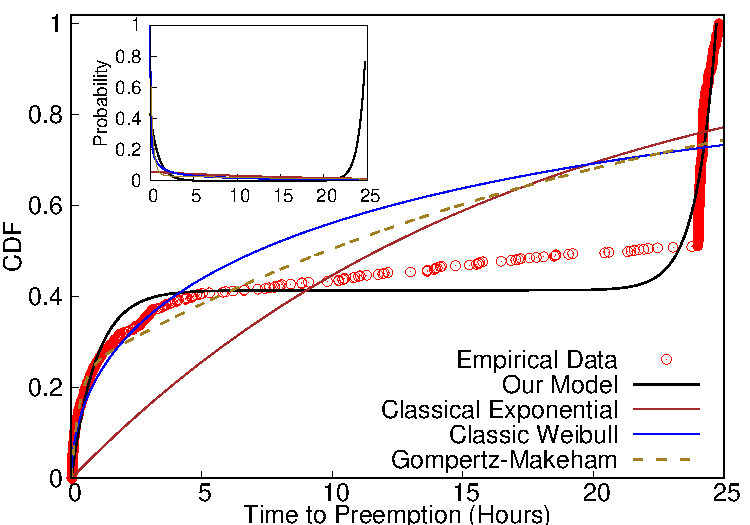
\includegraphics[width=0.47\textwidth]{../data/gnuplot-figures/sigmetrics-fig-cdf-prob-inset-time.pdf} 
  \caption{CDF of lifetimes of Google Preemptible VMs. Our proposed distribution for modeling the constrained preemption dynamics provides better fits to the empirical data compared to other failure distributions. Inset shows the probability density functions.}
  \label{fig:gcp1}
\end{figure}

To understand the nature of temporally constrained preemptions, we conducted the first empirical study of Google's Preemptible VMs, that have a fixed price and a maximum 24 hour lifetime.
Our empirical study is necessitated by the fact that the cloud operator (Google) does not disclose any other information about the preemption rates, and thus relatively little is known about the preemptions of these VMs, and as a result their performance.


We launched  1,516 Google Preemptible VMs of different types over a two month period (Feb--April 2019), and measured their time to preemption (i.e., their useful lifetime).\footnotemark
To ensure the generality of our empirical observations, VMs of different resource capacities were launched in a four geographical regions; during days and nights and all days of the week; and running different workloads. 
%
\footnotetext{We will release the complete preemption dataset for further analysis.} %Weaksauce 
%
A sample of over 100 such preemption events are shown in Figure~\ref{fig:gcp1}, which shows cumulative distribution function (CDF) of the VM lifetimes of the \texttt{n1-highcpu-16} VM in the \texttt{us-east1-b} zone. 
%enter the type of VM for which the data is shown
Note that the cloud operator (Google) caps the \emph{maximum} lifetime of the VM to 24 hours, and all the VMs are preempted before that limit. 

\begin{figure*}
  %\centering
  \subfloat[Preemption characteristics of different VM types. Larger VMs are more likely to be preempted.
  \label{fig:cdf-comparison}]
  {  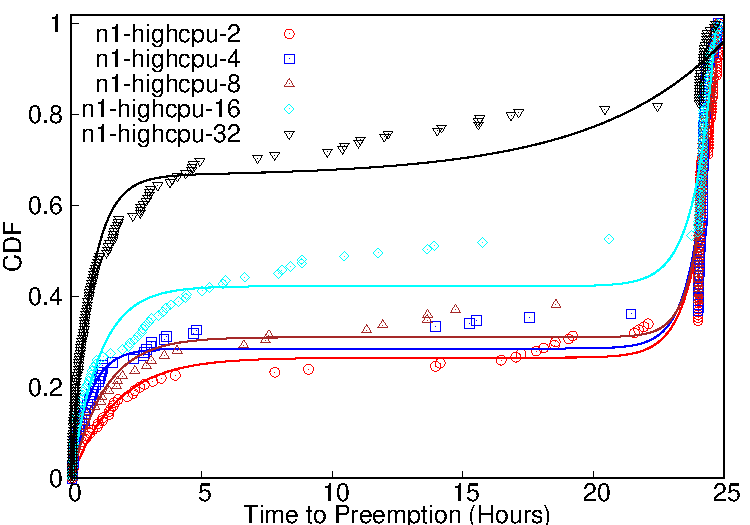
\includegraphics[width=0.3\textwidth]{../data/gnuplot-figures/sigmetrics-fig-vm-types.pdf} }
  \hfill
\subfloat[Variations due to time of day and workload. \label{fig:time-breakdown}]
{  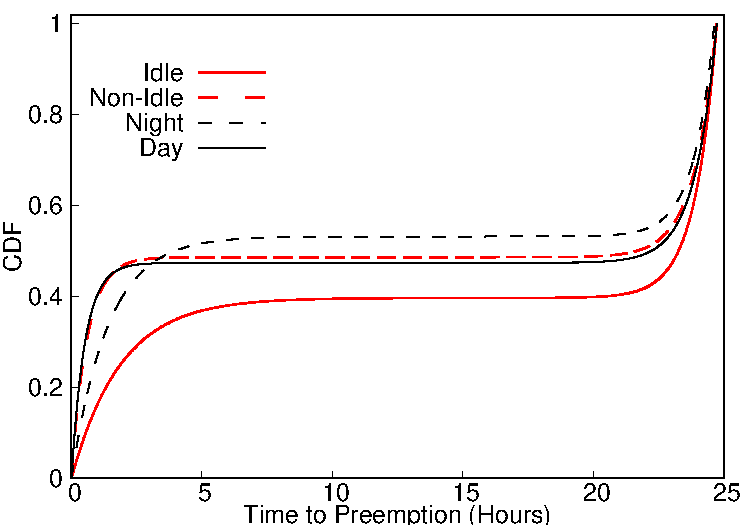
\includegraphics[width=0.3\textwidth]{../data/gnuplot-figures/sigmetrics-time-breakdown.pdf} }
\hfill
\subfloat[\textbf{n1-highcpu-16} in different regions. \label{fig:region-breakdown}]
{  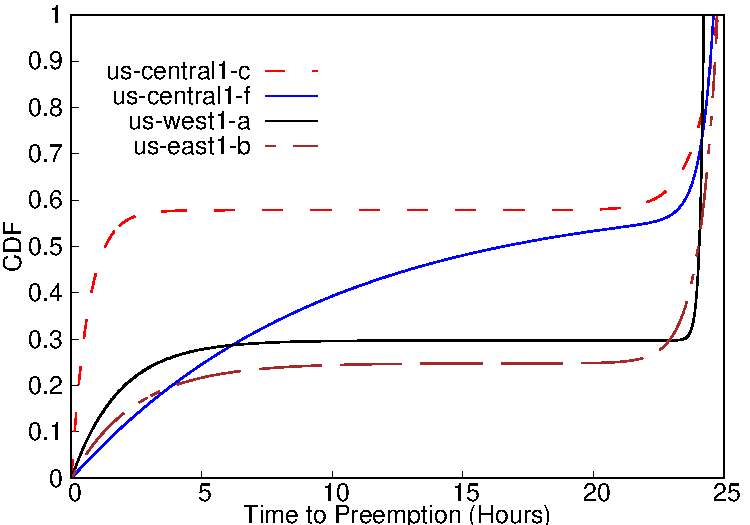
\includegraphics[width=0.3\textwidth]{../data/gnuplot-figures/sigmetrics-region-breakdown.pdf} }
\vspace*{-0.6cm}
\caption{Analysis of preemption characteristics by VM-type, region, time-of-day, and workload type.}
\label{fig:breakdown-all}
    \vspace*{\myfigspace}
\end{figure*}

\noindent \textbf{Observation 1:} \emph{The lifetimes of VMs are not uniformly distributed, but have three distinct phases.}

\noindent In the first (initial) phase, characterized by VM lifetime $t\in [0, 3]$ hours, we observe that many VMs are quickly preempted after they are launched, and thus have a steep rate of failure. The rate of failure (preemption rate) is the derivative of the CDF.
%; the rate of failure or preemptions can be obtained by taking the derivative of the CDF. 
In the second phase, VMs that survive past 3 hours enjoy a relatively low preemption rate over a relatively broad range of lifetime (characterized by the slowly rising CDF in Figure~\ref{fig:gcp1}).
The third and final phase exhibits a steep increase in the number of preemptions as the preemption deadline of 24 hours approaches.
The overall rate of preemptions is ``bathtub'' shaped as shown by the solid black line in the inset of Figure~\ref{fig:gcp1} (discussed in detail below).
%\it I think we should show the probability plot to exhibit the bath tub shape

%The preemption rate is ``bath tub'' shaped, with VMs that survive past 3 hours enjoying a relatively low preemption rate, and finally a steep increase in the number of preemptions as the preemption deadline (24 hours) approaches. 


\noindent \textbf{Observation 2:} \emph{The preemption behavior, imposed by the constraint of the 24 hour lifetime, is substantially different from conventional failure characteristics of hardware components and EC2 spot instances.}

\noindent In ``classical'' reliability analysis, the rate of failure  usually follows an exponential distribution $f(t) = \lambda e^{-\lambda t}$, where $\lambda=1/\text{MTTF}$.
Figure~\ref{fig:gcp1} shows the CDF ($=1-e^{-\lambda t}$) of the exponential distribution when fitted to the observed preemption data, by finding the distribution parameter $\lambda$ that minimizes the least squares error.
The classic exponential distribution is unable to model the observed preemption behavior because it assumes that the rate of preemptions is independent of the lifetime of the VMs, i.e., the preemptions are \emph{memoryless}.
%The primary reason is that the exponential distribution assumes that the \vj{the rate of preemptions is independent of the lifetime of the VMs} (preemptions are \emph{memoryless}), which does not hold true when there is a fixed upper bound on the lifetime, as is the case for Google Preemptible VMs. \vj{In other words, the conventional approach is insufficient to model constrained preemption dynamics.}
%We attribute this deficiency to the central assumption made in the underlying reliability theory principles that leads to the classical exponential distribution: the rate of preemptions is independent of the lifetime of the VMs, in other words, the preemptions are \emph{memoryless}.
This assumption breaks down when there is a fixed upper bound on the lifetime. %, as is the case for Google Preemptible VMs.%, and the conventional approach becomes insufficient to model this constrained preemption dynamics. 

\noindent \textbf{Observation 3:} \emph{The three preemption phases and associated bathtub shaped preemption probability are general, universal characteristics of Preemptible VMs.}

In general, the preemption dynamics of a VM are determined by the supply and demand of VMs of that \emph{particular} type.
Thus, our empirical study looked at preemptions of VMs of different sizes, in different geographical zones, at different times of the day, and running different workloads (Figure~\ref{fig:breakdown-all}).
In all cases, we find that there are three distinct phases associated with the preemption dynamics giving rise to the bathtub shaped preemption probability. 
We argue that this is not a coincidence, but may be a result of practical and fundamental outcomes of cluster management policies. 

While the actual specific preemption policy is up to the cloud operator, we will show that the bathtub behavior has benefits for applications. 
%The bathtub behavior results in a high rate of failure initially. 
For applications that do not incorporate explicit fault-tolerance (such as checkpointing), early preemptions result in less wasted work than if the preemptions were uniformly distributed over the 24 hour interval.
Furthermore, the low rate of preemptions in the middle periods allows jobs that are smaller than 24 hours to finish execution with only a low probability of failure, once they survive the initial preemption phase. 
We evaluate the performance of applications with bathtub shaped preemptions in Section~\ref{sec:eval}. 
%
In addition to being beneficial to applications, we also conjecture that the bathtub behavior may be  a \emph{fundamental} and general characteristic of constrained preemptions, which we show later in Section~\ref{subsec:stat-mech}. 
%system where events are randomly distributed in a finite interval later in Section~\ref{subsec:stat-mech}. 
%
%Intriguingly, we can analyze such temporally constrained preemptions through a statistical mechanics framework, and we elaborate on this connection later in Section~\ref{subsec:statmech}.


\noindent \textbf{Observation 4:}\emph{ Larger VMs have a higher rate of preemptions.}

Figure~\ref{fig:cdf-comparison} shows the preemption data from five different types of VMs in the Google Cloud \texttt{n1-highcpu-\{2,4,8,16,32\}}, where the number indicates the number of CPUs.
All VMs are running in the \texttt{us-central1-c} zone. 
We see that the larger VMs (16 and 32 CPUs) have a higher probability of preemptions compared to the smaller VMs.
While this could be simply due to higher demand for larger VMs, it can also be explained from a cluster management perspective. 
Larger VMs require more computational resources (such as CPU and memory), and when the supply of resources is low, the cloud operator can quickly reclaim a large amount of resources by preempting larger VMs.
This observed behavior aligns with the guidelines for using preemptible VMs that suggests the use of smaller VMs when possible~\cite{preemptible-documentation}. 

\noindent \textbf{Observation 5:} \emph{Preemptions exhibit diurnal variations, and are also affected by the workload inside the VM.}

From Figure~\ref{fig:time-breakdown}, we can see that VMs have a slightly longer lifetime during the night (8 PM to 8 AM) than during the day.
This is expected because fundamentally, the preemption rates are higher during periods of higer demand. 
%
We also notice that completely idle VMs have longer lifetimes than VMs running some workload.
Presumably, this could be a result of the lower resource utilization of idle VMs being more amenable to resource overcommitment, and result in lower preemptions. 

\begin{figure}
  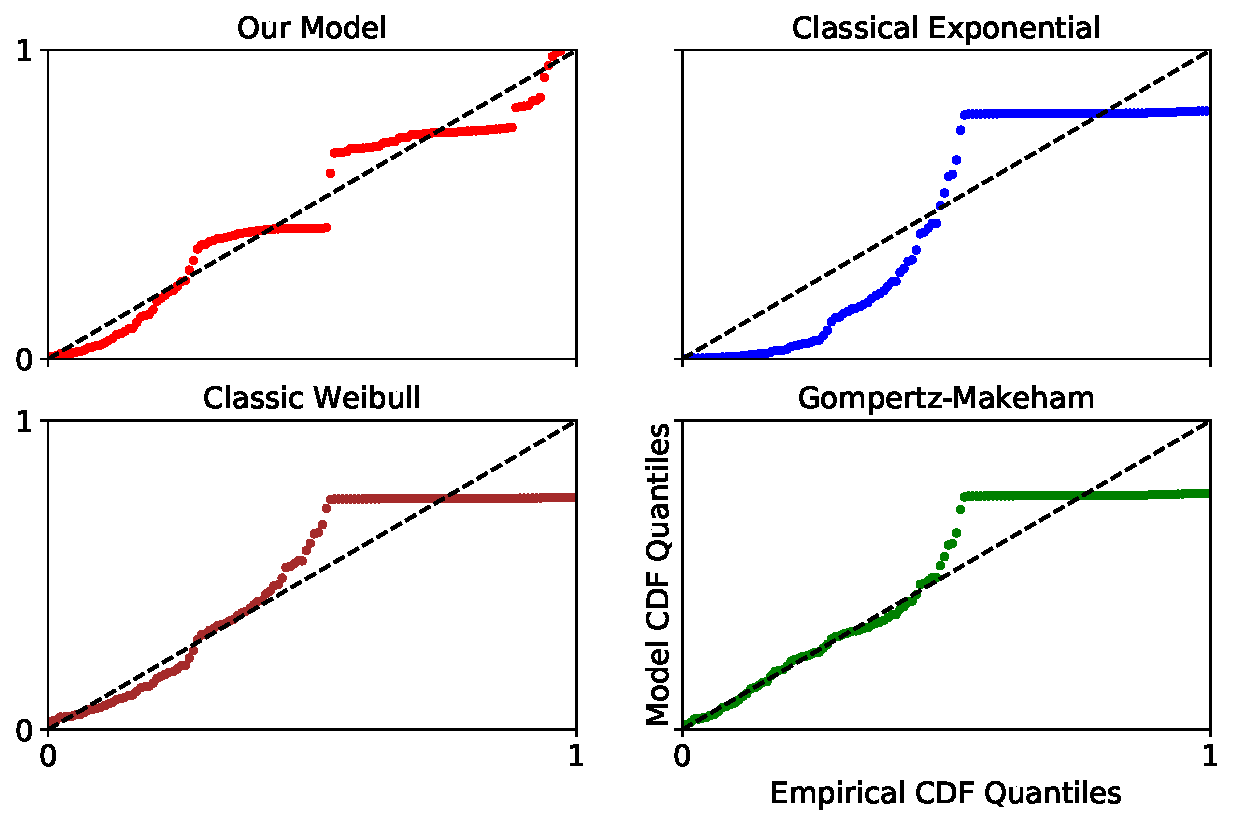
\includegraphics[width=0.4\textwidth]{../graphs/QQ.pdf}
    \vspace*{-5pt}
  \caption{QQ plot of different preemption models. Existing models are unable to capture all the preemption phases.}
  \label{fig:QQ}
  \vspace*{-5pt}
\end{figure}

%being more amenable to resource overcommitment, and therefore don

%%%%%%%%%%%%%%%%%%%%%%%%%%%%%%%%%%%%%%%%%%%%%%%%%%%%%%%%%%%%%%%%%%%%%%

\vspace*{\subsecspace}
\subsection{Failure Probability Model}
\label{subsec:analytical-model}

%Based on our empirical analysis of preemptions,  
We now develop an analytical probability model for finding a preemption at time $t$ (preemption dynamics) that is faithful to the empirically observed data and provides a basis for developing running-time and cost-minimizing optimizations. %
Modeling preemptions constrained by a finite deadline raises many challenges for existing preemption models that have been used for other transient servers such as EC2 spot instances. 
We first discuss why existing approaches to preemption modeling are not adequate, and then present our closed-form probability model and associated reliability theory connections. 

%How to avoid sounding like the background section?

\subsubsection{Inadequacy of existing failure distributions}

Spot instance preemptions have been modeled using exponential distribution~\cite{bid-cloud, hotcloud-not-bid, flint}, which is the default in most reliability theory applications. 
However, the strict 24 hour constraint and the distinct preemption phases are not compatible with the memoryless properties of the exponential distribution. 
%
To describe failures (preemptions) that are not memoryless (i.e., increasing or decreasing failure rate over time), the classic Weibull distribution with CDF $F(t)=1-e^{-(\lambda t)^k}$ is often employed. However, the Weibull distribution is also unable to fit the empirical data (Figure~\ref{fig:gcp1}) and especially unable to model the sharp increase in preemptions near the 24 hour deadline. 

For constrained preemptions, the increase in failure rate as modeled by the Weibull distribution is not high enough.
Other distributions, such as Gompertz-Makeham, have also been used for modeling bathtub behavior, especially  for actuarial use-cases~\cite{missov2013gompertz}. 
The key idea is to incorporate an exponential aging process, which is used to model human mortality.
The CDF of the Gompertz-Makeham distribution is given by $F(t) = 1 - \exp\left(-\lambda t - \dfrac{\alpha}{\beta}(e^{\beta t} - 1) \right)$
  and is fitted to the data in Figure~\ref{fig:gcp1}, and is also unable to provide a good model for the observed preemption data. 

%Specifically, it is unable to model the bathtub preemption rate and the different preemption phases, and 


%We also analyze other distributions used for modeling bathtub failures from reliability and actuarial theory in Figure \textbf{XXX}.


The non-trivial bathtub-shaped failure rate of Google preemptible VMs (Figure~\ref{fig:gcp1}) requires models that capture the sudden onset of the rise in preemptions near the deadline.
From an application and transiency policy perspective, the preemption model must provide insights about the phase transitions, so that the application can adapt to the sharp differences in preemption rates.
%
For example, the preemption model should be able to warn applications about impending deadline, which existing failure distributions cannot account for. 
% which imposes a dynamics that is more akin to a constrained dynamics problem as opposed to dynamics characterized with a gradually rising failure rate.
Thus, not only is it important to minimize the total distribution fitting error, it is also important to capture the changes in phase.
However, as we can see from Figure~\ref{fig:QQ}, existing distributions are unable to capture the effects of the deadline and the phases of the preemptions, and a new modeling approach is needed, which we develop next.  

\subsubsection{Our  model}
\label{subsec:preemption-model}


%This is especially important from a policy design perspective, as the ``phase changes'' in preemption behavior can greatly affect the failure probability and performance of applications.
%Our new model, informed by the cumulative distribution of lifetimes that has multiple distinct temporal phases, addresses this need.

Our failure probability model seeks to address the drawbacks of existing reliability theory models for modeling constrained preemptions. 
The presence of three distinct phases exhibiting non-differentiable transition points (sudden changes in CDF near the deadline, for example) suggests that for accurate results, models that treat the probability as a step function (CDF as a piecewise-continuous function) should be employed. However, this limits the range of model applicability and general interpretability of the underlying preemption behavior. Our goal is to provide a broadly applicable, continuously differentiable, and informative model built on reasonable assumptions.  

We begin by making a key assumption: the preemption behavior arises from the presence of \emph{two} distinct failure processes.
%that give rise to a new probability distribution characterizing the preemptions and the observed CDF, and ensure the dependence of the rate of failure on the VM lifetime. 
The first process dominates over the initial temporal phase and yields the classic exponential distribution that captures the high rate of early preemptions.
The second process dominates over the final phase near the 24 hour maximum VM lifetime and is assumed to be characterized by an exponential term that captures the sharp rise in preemptions that results from this constrained lifetime. 
%Generally, these two processes jointly determine the dynamics of preemptions during the middle phase where a relatively constant or a slowly rising number of preemptions with time is observed.
%; in practice, based on the fits to the empirical data, we observe the first process to dominate over the second during this phase as well. 

%The first two phases are reasonably captured by the classic exponential distribution. In order to model the overall observed empirical CDF, we add another term that captures the failure process near the 24 hour maximum VM lifetime,  and construct a \emph{new} probability distribution. 
%
%we develop a \emph{new} probability distribution that is composed by blending two failure processes that act on different temporal phases over the 24 hour maximum lifetime of the VMs. 
%
%We write the general form of our blended preemption CDF as follows:

Based on these observations, we propose the following general form for the CDF:

\vspace*{\subsecspace}
\begin{equation}
  \label{eq:blend1}
  \boxed{
  \mathscr{F}\left(t\right) = A\left(1-e^{-\frac{t}{\tau_1}} + e^{\frac{t-b}{\tau_2}}\right)}
  \end{equation}
\noindent where $t$ is the time to preemption, $1/\tau_1$ is the rate of preemptions in the initial phase, $1/\tau_2$ is the rate of preemptions in the final phase, $b$ denotes the time that characterizes ``activation'' of the final phase where preemptions occur at a very high rate, and $A$ is a scaling constant. 
%
The model is fit to data for $0 < t < L$, where $L \approx 24$ hours represents the temporal interval (deadline).
Combination of the 4 fit parameters ($\tau_1, \tau_2, b$, and $A$) are chosen to ensure that boundary condition $\mathscr{F}(0) \approx 0$ is satisfied.
%and $\mathscr{F}(L) \approx 1$. 
%%When not used as a fit parameter, $A$ is chosen as $A = 1/(1-e^{-\frac{L}{\tau_1}} + e^{\frac{L-b}{\tau_2}})$ to ensure $F(L) = 1$, yielding results similar to the 4 parameter fit. 
In practice, typical fit values yield $b \approx 24$ hours, $\tau_1 \in [0.5, 0.8] $, $\tau_2 \approx 1$ hour, and $A \approx 0.7$.



%\vikram{check, and provide typical fit values for all these parameters as well as their range extremes. ideally, you want to fit with A set to the above expression to avoid any $\mathscr{F}(t)$ or $p(t)$ > 1 scenarios. turns out that having A is important in reliability analysis -- check next column}


%of  0 $\approx 0$ premptions.
%used to scale the CDF to ensure that the initial conditions ($F(0)=0$) are met.

For most of its life, a VM sees failures according to the classic exponential distribution with a rate of failure equal to $1/\tau_1$ -- this behavior is captured by the $1-e^{-t/\tau_1}$ term in Equation~\ref{eq:blend1}. 
%However, this does not capture the finite lifetime of the VM imposed by the cloud operator.
As VMs get closer to their maximum lifetime imposed by the cloud operator, they are reclaimed (i.e., preempted) at a high rate $1/\tau_2$, which is captured by the second exponential term, $e^{(t-b)/\tau_2}$ of Equation~\ref{eq:blend1}. 
Shifting the argument ($t$) of this term by $b$ ensures that the exponential reclamation is only applicable near the end of the VM's maximum lifetime and does not dominate over the entire temporal range. 
%As noted before, $1/\tau_2$ is the rate of this reclamation. 

The analytical model and the associated  distribution function $\mathscr{F}$ introduced above provides a much better fit to the empirical data (Figure~\ref{fig:gcp1}) and captures the different phases of the preemption dynamics through parameters $\tau_1, \tau_2, b$, and $A$. These parameters can be obtained for a given empirical CDF using least squares function fitting methods (we use scipy's \texttt{optimize.curve\_fit} with the dogbox technique~\cite{scipy-fit}). The failure or preemption rate can be derived from this CDF as:
\begin{equation}
  \label{eq:failrate}
    \vspace*{\eqnspace}
f(t) = \dfrac{d \mathscr{F}(t)} {dt} = A \left(\dfrac{1}{\tau_1}e^{-t/\tau_1} + \dfrac{1}{\tau_2}e^{\frac{t-b}{\tau_2}}\right).
\end{equation}
$p(t)$ vs. $t$ yields a bathtub type failure rate function for the associated fit parameters (inset of Figure~\ref{fig:gcp1}).
%In the next section, we use this analytical model for optimizing cloud resource selection to run scientific computing applications at low cost and shorter running (turnaround) times.


In the absence of any prior work on constrained preemption dynamics, our aim is to provide an interpretable model with a minimal number of parameters, that provides a sufficiently accurate characterization of observed preemptions data. 
%As is evident from Figure~\ref{fig:gcp1}, our model shows deviations from the data near the halfway point within the 24 hour lifetime. 
Further generalization of this model to include more failure processes would introduce more parameters and reduce the generalization power. 
%Exploring other approaches of modeling bathtub-type failure rates (e.g., exponential Weibull distributions) \cite{mudholkar1993exponentiated,crevecoeur1993model} is part of our future work. 


\subsubsection{Reliability Analysis}
\label{subsec:reliability}

We now analyze and place our model in a reliability theory framework. 
%

\noindent \textbf{Expected Lifetime:} Our analytical model also helps crystallize the differences in VM preemption dynamics, by allowing us to easily calculate their expected lifetime. 
More formally, we define the expected lifetime of a VM as: 
\begin{equation}
  \label{eq:expected-lifetime}
E[L] =  \int_{0}^{24} t {f}(t)~dt =  -A(t+\tau_1)e^{-t/\tau_1} + A(t-\tau_2) e^{\frac{t-b}{\tau_2}} \biggr\rvert_{0}^{24}
\end{equation}
where $f(t)$ is the rate of preemptions of the VM (Equation~\ref{eq:failrate}).
%= \dfrac{d \mathscr{F}(t)} {dt} = A \left(\dfrac{1}{\tau_1}e^{-t/\tau_1} + \dfrac{t-b}{\tau_2}e^{\frac{t-b}{\tau_2}}\right) $ 
%
%Since preemptions require restarting a job and increase the job completion time, it may be more prudent to select transient VMs with higher expected lifetimes.

This expected lifetime can be used in lieu of MTTF, for policies and applications that require a ``coarse-grained'' comparison of the preemption rates of servers of different types, which has been used for cost-minimizing server selection~\cite{flint}. 

%We use the analytically derived expected lifetimes of VMs of different types in \sysname when selecting the ``best'' VM type for a given bag of jobs. This server selection is a key part of \sysname design. 

\noindent \textbf{Hazard Rate:}
The hazard rate $\lambda(t)$ governs the dynamics of the failure (or survival) processes. It is generally defined as $\lambda(t) = \frac{g(t)}{S(t)}$, often expressed via the following differential equation (rate law):
\begin{equation}\label{eq:hazard}
\frac{dS(t)}{dt} = -\lambda(t) S(t)
\end{equation}
%$\lambda(t) = \frac{f(t)}{S(t)}$ \vikram{this was inverted, I fixed. double check please}, 
where $S(t) = 1 - F(t)$ is the survival function associated with a CDF $F(t)$, and $g(t)=dF(t)/dt$ is the failure probability function (rate) at time $t$. The survival function indicates the amount of VMs that have survived at time $t$.
The hazard rate can also be directly expressed in terms of the CDF as follows: $1-F(t) = \exp{\int_0^t{-\lambda(x) ~dx}}$. 
The exponential distribution has a constant hazard rate $\lambda$.
The Gompertz-Makeham distribution has an increasing failure rate to account for the increase in mortality, and its hazard rate is accordingly non-uniform and given by $\lambda(t) = \lambda + \alpha e^{\beta t}$.

Since we model multiple failure rates and deadline-driven preemptions, our hazard rate is expected to increase with time. Defining the survival function for our model: $S = 1 - \mathscr{F}$, and using Eq.~\ref{eq:hazard} yields the hazard rate associated with our model: 
%$\lambda(t) = \dfrac{- r_1 e^{- r_1 t} - r_2 e^{r_2 (t - b)}}{e^{- r_1 t} - e^{r_2 (t - b)}}$. 
% missing minus sign in the above equation
\noindent 
\begin{equation}
  \label{eq:hmodel}
  \lambda %= r_2 + \bar{r} \left( \dfrac{1}{1 - e^{- r_2 b} e^{\bar{r} t}}\right)
  %= \dfrac{r_1 + r_2 e^{- r_2 b} e^{\bar{r} t}}{1 - e^{- r_2 b} e^{\bar{r} t}}.  
  = \dfrac{r_1 e^{- r_1 t} + r_2 e^{r_2 (t - b)}}{1/A - 1 + e^{- r_1 t} - e^{r_2 (t - b)}}
\end{equation}
where we have introduced $r_1 = 1/\tau_1$, $r_2 = 1/\tau_2$ to denote the rates of preemptions associated with initial and final phases respectively.

%\vikram{without the A term, hazard rate becomes negative for the older expression you had when $t > b r2 / (r1+r2)$. that is for t roughly greater than b/2, which is for more than 12 hours. hazard rate can never be negative.}
%Here we have introduced the sum of the two failure rate constants, $\bar{r} = r_1 + r_2$, to simplify the expression. \vikram{check}

%Employing the value for $A$ resulting from ensuring (via fit or by force) that our CDF goes to 1 at $t = L$ (where $L$ is 24 hours), we find

% \begin{equation}
%   \label{eq:hmodel2}
%   \lambda %= r_2 + \bar{r} \left( \dfrac{1}{1 - e^{- r_2 b} e^{\bar{r} t}}\right)
%   %= \dfrac{r_1 + r_2 e^{- r_2 b} e^{\bar{r} t}}{1 - e^{- r_2 b} e^{\bar{r} t}}.  
%   = \dfrac{r_1 e^{- r_1 t} + r_2 e^{r_2 (t - b)}}{e^{r_2 (L - b)}  - e^{- r_1 L} + e^{- r_1 t} - e^{r_2 (t - b)} }
% \end{equation}

Recall that the sharp increase in preemption rate only happens close to the deadline, which means that $b \lesssim L$. Thus, when $0 < t \ll b$, we get $\lambda(t) \approx r_1$, mimicking the hazard rate for the classic exponential distribution.
As $t$ approaches and exceeds $b$ (i.e., $b\lesssim t < L$), the increase in the hazard rate due to the second failure process kicks in, accounting for the deadline-driven rise in preemptions. Note that our hazard rate satisfies $\lambda(t) \ge 0$ for $0<t<L$.

% For ease of exposition, we can write this as:

% \begin{equation}
%  \label{eq:hmodelsimple}
% \lambda =  \dfrac{r_1 + \gamma_1 e^{\delta (t-b)}}{1 - \gamma_2 e^{\delta (t-b)}}
% \end{equation}
% 
% We note that the numerator is  similar to the hazard rate associated with Gompertz-Makeham distribution.
% The key difference is the $1-\gamma_2 e^{t-b}$ factor in the denominator. 
% Recall that the sharp increase in preemption rate only happens close to the deadline, which means that $b \leq 24$. Thus, when $t < b$, we get a conventional $\lambda = r_1$, or the classic exponential distribution.
% As $t$ approaches and exceeds $b$, the increase in failure rate kicks in, accounting for the deadline-driven rise in preemptions. 



% We emphasize that our motivation is to develop an interpretable \emph{minimal} model that provides a sufficiently accurate description of the observed constrained preemption dynamics of Google VMs with a minimal number of meaningful parameters. 
% As is evident from Figure~\ref{fig:gcp1}, $\mathscr{F}$ shows deviations from the data near the halfway point within the 24 hour lifetime.
% Further generalization of this model to include more failure processes, which would introduce more parameters, or exploring other approaches of modeling bathtub-type failure rates (e.g., exponential Weibull distributions) \cite{mudholkar1993exponentiated,crevecoeur1993model} may yield alternate model descriptions that capture the data with higher accuracy.


%PXXX part of future work? 

%characterized by failure rates and activation times (like $b$). 
%and reduce the predictive power and simplicity of the model. 
%We also note that approaches (e.g., exponential Weibull distributions) to model bathtub-type failure rates have been proposed in the literature  \cite{mudholkar1993exponentiated,crevecoeur1993model}.
%These methods did not perform better than our model resulting in parameter variables and values that were relatively difficult to interpret; this could likely be due to the unique constraint-driven failures in preemption dynamics as opposed to aging-related increasing failure rate considered in previous work. 

\subsection{Insights on the bathtub shape distribution}
\label{subsec:stat-mech}

For constrained preemptions, one might expect to see uniformly distributed preemptions with a probability $1/L$ over $[0, L]$. 
However, as our empirical analysis shows, the preemption distribution is baththub shaped.
Interestingly, we can show using exact analytical arguments that non-uniform, baththub distributions are in fact a \emph{general} characteristic of systems with constrained preemptions, modulo some assumptions. 

\begin{lemma}\label{lemma:1}
  Consider $N$ randomly distributed preemptions over an interval $[0, L]$.
  Assume that each preemption takes $w > 0$ time-units to perform, and preemptions cannot overlap, i.e, they occur in a mutually exclusive manner.
  Then, there exists $\epsilon > 0$ such that  $P(L-\epsilon) > \frac{1}{L}$, where 
 $P(t)$ is the probability of finding a preemption at time $t$. 
\end{lemma}


\begin{proof}
We first make some preliminary remarks and introduce concepts necessary to complete the proof. 

Firstly, mutual exclusion of preemptions implies that there is a finite non-zero waiting time $w>0$ between preemptions. 
For $N$ preemptions to occur within $L$ interval, evidently, we must have $Nw < L$. Also, while $w >0$, the time to perform the preemption is generally expected to be much smaller than the total time interval $L$.
$N$ preemptions occupy a ``temporal volume'' of $Nw$ (volume here represents the one-dimensional volume). We assume that while a preemption may start at $t=0$, the last preemption must finish by $t = L$. Thus, the amount of free or excluded ``temporal volume'' available within the constrained system is $L_e = L - w - (N-1)w = L - Nw$.
The idea of excluded volume is central in physics and materials engineering where it underpins the origin of entropic or steric forces in material systems \cite{krauth2006statistical,jing2015ionic}. 

Secondly, we note that the system of $N$ preemptions within a constrained deadline of interval $L$ maps \emph{exactly} to a well known and analytically solvable system in classical statistical mechanics, the Tonks gas model \cite{tonks}, where one considers a system of $N$ hard-spheres of diameter $w$ to move along a line segment of length $L$. The structural quantities associated with this system including the probability of finding a sphere at position $x$ within the interval $L$ are computed by evaluating the partition function of the system, which essentially measures the number of valid system configurations \cite{krauth2006statistical}. Employing this mapping and the associated statistical mechanics tools, the original model of non-overlapping (interacting) preemptions can be mapped to a system of $N$ overlapping (non-interacting) preemptions, each allowed to access an excluded volume of $L_e$, and the number of valid configurations is given by the partition function $Z_N = L_e^N$. For the case of $N$ preemptions, we have $Z_N = (L- Nw)^N$.

We are interested in calculating the probability that a preemption starts at time $t=L-w$, i.e., $P(L-w)$. Given that the time to perform the preemption $w$ is generally expected to be much smaller than the total time interval $L$, $P(L-w)$ is the probability of finding a preemption near the deadline. The assumption of mutually exclusive preemptions implies that no other preemption can be found for $t > L - w$, that is, $P(t> L-w) = 0$. Hence, the remaining $N-1$ preemptions must occur such that the last of those finish by $t=L-w$ (the preemption at time $L-w$ essentially sets an effective deadline for the other $N-1$ preemptions). The number of ways this can happen is given by the partition function $Z_{N-1} = L_e^{N-1}= (L-2w - (N-2)w)^{N-1} = (L - Nw)^{N-1}$, where $L_e = L - Nw$ is the corresponding excluded temporal volume accessible to each of the $N-1$ preemption. It is interesting to note that the excluded volume in this case is the same as that of the original $N$ preemption system: this fortuitous result arises because the reduction in available volume to place the preemptions is commensurate with the need to place $N-1$ preemptions instead of $N$.

The probability $P(L-w)$ is obtained as the ratio of the valid configurations given by the two partition functions computed above.
That is, 
$P(L-w) = Z_{N-1}/ {Z_N} = \frac{1}{L - Nw} > \frac{1}{L}$ , since $N \geq 1$ and $w>0$. Choosing $\epsilon = w > 0$ completes the proof.


%We begin by counting the total number of configurations available to place $N$ preemptions in the constrained temporal ``volume'' $L$. 
%The number of configurations one preemption can generate is proportional to the excluded volume available, i.e., $L-Nw$.
%For $N$ preemptions, the number of configurations grows exponentially and is proportional to the volume of the $N$-dimensional hypercube: $Z = (L-Nw)^N$. 
%This computation of the number of valid system configurations is in fact the partition function of the system in statistical mechanics~\cite{krauth2006statistical}. 

%Given the condition of mutually exclusive preemptions, we note that if we assume that there is a preemption at $t=L-w$, then $P(t> L-w) = 0$.
%For this case, the available, valid, non-overlapping configurations are proportional to the temporal volume accessible in the $N-1$ dimensional hypercube to $N-1$ preemptions: $Z_{1} = (L-w-(N-1)w)^{N-1} = (L-Nw)^{N-1}$. 

%The probability of finding 1 preemption near the deadline at $t=L-\epsilon$ when $\epsilon \in [w/2, w)$ is given as the ratio of the two computed volumes.
%That is, $P(L-\epsilon) = \frac{Z_1}{Z} = \frac{1}{(L - N\epsilon)} > \frac{1}{L}$ , since $N \geq 1$ and $\epsilon>0$. 
\end{proof}

By symmetry arguments, the above lemma is in fact valid for both the end points of the interval, i.e., $P(\epsilon) > \frac{1}{L}$.
Thus, the probability of preemption is higher near the end points (deadline) than the average preemption probability of $1/L$, and we get a bathtub shaped distribution.
Thus, the bathtub distribution can be considered to be a general artifact of constrained preemptions. Of course, the empirical preemption distribution is determined by the cloud platform's policies and supply and demand, and we elaborate more about the generality of our model and observation in Section~\ref{sec:discussion}. 

% How ?
%Crucial to our The assumption of preemption events

For the above proof, we assumed that each preemption event occurs over a timespan of $w$, which is determined by the preemption warning that the cloud platform provides (which is 30 seconds for Google Preemptible VMs and 120 seconds for Amazon EC2 spot instances). 
Preempting a VM and reclaiming its resources involves manipulating the cluster-management state, and mutually exclusive preemptions may be convenient for cluster management, since serializing VM preemptions makes accounting and other cluster operations easier.
From an application standpoint, non-overlapping preemptions are also beneficial, since handling multiple concurrent preemptions is significantly more challenging~\cite{exosphere}. 





\begin{comment}
\subsection{Elsewhere: Role of Cloud Providers: Analogy to Constrained Physical Systems}

The bathtub-shaped distribution of the preemption probability is essential to capture the empirical data with higher accuracy compared to other models. We want to probe the following question now: how much of this unique shape is enforced by the cloud provider, and how much is dictated by assuming that (akin to other cloud providers such as EC2), preemptions of Google Preemptible VMs are placed along the timeline of 24 hours with uniform probability? We make the question more precise and inject a relatively harmless assumption: if the cloud provider decides to ``place'' $N$ preemptions within the temporal boundary of interval $L$ with flat probability distribution ($\mathscr{P}(e_1, e_2, \ldots e_N)$ = 1 whenever legal) such that the preemptions are mutually exclusive (that is there is a finite non-zero waiting time between preemptions), what is the probability of finding a preemption at time $t$? Naively, deducing from $\mathscr{P}$, one may expect $p(t)$ to be 1 for $t\in L$, or a constant (flat) distribution. However, intruigingly, this is not true. Thus, as we discuss in more detail below, the cloud provider may have the simplest of preemption policies implemented at their end, and yet give rise to the relatively complex and non-trivial probability to preemption. 

To understand the above assertions with a simple example that sheds further insights into the origins of the bathtub-shaped distribution, we discuss analogous questions in the context of general physical systems of constrained (confined) particles.
These systems are generally analyzed using the theoretical framework of statistical mechanics often complemented with associated particle dynamics simulations. We choose an exactly solvable and simple system of hard (non-overlapping) particles (or beads) confined to move in one dimension within a finite spatial interval to draw interesting connections. 

A simple mapping from the system of temporally-constrained preemptions in the cloud to the system of spatially-constrained particles within one-dimensional confinement can be established by assuming that the cluster management policy requires mutually exclusive preemptions.
This assumption helps cluster management by serializing VM preemptions and making cluster operations easier, and it reduces the challenges associated with reacting to simultaneous preemptions. 
The preemption events become hard particles that cannot overlap. The preemption probability distribution gets mapped to the density of $N$ particles, each modeled as a one-dimensional ``sphere'' of width $\sigma$, confined in a 1-dimensional interval (line segment) of length $L$. $L$ can be considered as corresponding to the deadline interval of 24 hours. $\sigma$ is equivalent to the length of the critical section, which is related to the preemption warning (30 seconds for Google PVMs). 

The particles are placed, one after another, at random positions. Configurations where any overlap is generated are not included. Thus particles will be placed with a flat probability distribution.
The question we are trying to simulate with this set up is the familiar one noted above: what is the probability $p(x)$ of finding a preemption at time $x$?

This problem can be solved by first defining a partition function for the system. And doing some neat math.

Present the solution

This distribution is \emph{not} uniform over the interval, but is higher towards the ends of the interval---analogous to the bath-tub shaped nature of preemptions! 

Discuss more.

We thus draw a few critical observations.
An immediate inclincation may be to attribute the observed non-trivial bathtub-shaped preemption probability function to a uniquely designed and structured operational policy of the cloud provider. However, the above analysis shows that even with the vanilla operational policy of placing preemptions with a uniform probability distribution, the finite excluded temporal volume of preemptions in conjunction with the relatively short deadline (which together imply a high average preemption rate) enforce a bathtub-shape-like distribution for finding a preemption at time $t$. Clearly, this does not provide all the subtle features observed in the preemption data as well as the failure model. But even there, it enables to gauge the extent to which the provider has changed the policy on top of the simplest possible implementation.

The analytical framework suggests that the bath-tub shape of the probability distribution is the key characteristic of constrained preemptions.
Therefore, our approach will remain relevant in the face of future changes in preemption characteristics due to changes in cloud usage and operational policies.

\end{comment}

%These systems underlie a variety of phenomena in chemical and materials engineering applications such as ions confined in nanochannels \cite{jing,solis}. 

%In addition to empirically-informed reliability models for preemptions, we also seek to understand \emph{why} their distribution is bathtub shaped in order to provide a mechanistic understanding of preemptions and enhance the model interpretability and generalizability. 
%Our key insight is that the problem of analyzing constrained preemptions can be ``mapped'' to an equivalent problem in statistical mechanics of a physical system, and we can use the theoretical and analytical framework of statistical mechanics to develop a broader understanding of preemptions. 
%This connection to statistical mechanics is given below. 
%To this end, we propose to ``map'' the problem of constrained preemptions to an equivalent problem of constrained many particle physical systems that can be analyzed employing the general theoretical framework of statistical mechanics.

%A simple mapping can be established by assuming that the cluster management policy requires mutually exclusive preemptions.
%This assumption helps cluster management by serializing VM preemptions and making cluster operations easier, and it reduces the challenges associated with reacting to simultaneous preemptions. The preemption events become hard particles that cannot overlap. The probability distribution of $N$ constrained preemption events gets mapped to the density of $N$ randomly distributed particles confined in a 1-dimensional interval of length $L$ (analogous to 24 hours). 
%The particle size is equivalent to the length of the critical section, which is related to the preemption warning (30 seconds for Google PVMs).
%Finding the distribution of non-overlapping (i.e., hard) particles is a central problem in statistical mechanics [5].
%Interestingly, the distribution of particles in a confined interval can be obtained analytically via the exact closed-form expression of the so-called partition function (a common statistical mechanical quantity useful for obtaining the microscopic understanding of macroscopic phenomena).
%This distribution is \emph{not} uniform over the interval, but is higher towards the ends of the interval---analogous to the bath-tub shaped nature of preemptions! 

%The analytical framework suggests that the bath-tub shape of the probability distribution is the key characteristic of constrained preemptions.
%Therefore, our approach will remain relevant in the face of future changes in preemption characteristics due to changes in cloud usage and operational policies.


% \subsection{EC2 spot instances}

% The earliest form of transient cloud instances.
% In addition to having dynamic availability, also have dynamic pricing.
% ``Classic'' spot instances had price determining the availability, and thus a large amount of work was devoted to bidding and analyzing the prices.

% However a recent change to the spot prices no longer allows these assumptions, rendering it impossible to obtain the \emph{exact} availability information from the prices alone.


% \subsection{Google Preemptible VMs}

% Launched in 2015.
% Flat-rate discount of 80\% compared to on-demand servers.
% Interesting availability SLA: the maximum lifetime is 24 hours, and can be preempted earlier as well.

% In this paper we will look at these preemptible VMs and show how to model their availability.
% Given the inability to use EC2 prices, we believe that our approach is more generalizable and robust.


% There are some distinguishing characteristics of GCP preemptible VMs that makes their failure modeling challenging.
% First is their flat pricing and no other signalling information about their preemption rates (MTBFs) that makes server selection difficult.

% \textbf{Modeling Failure Behavior of Preemptible VMs}
% CDF is ``sigmoid'' shaped.
% $P=R*np.sinh((t-t0)/tau) + C$ with a very low $R=10^{-6}, t_0=12, \tau=0.9, C=0.36$

% Basically, this is a mixture of two distributions, the standard exponential distribution, which we call the stabilization rate and an exponentially increasing reclamation rate.

% Preemptible VMs have three availability phases.

% There are many early deaths, then a period of low failure rates, and then the failure rate is exponential with a positive exponent to enable the cloud provider to reclaim the VMs within the deadline (24 hours in the case of Google's Preemptible VMs).








%%% Local Variables:
%%% mode: latex
%%% TeX-master: "paper"
%%% End:


\section{Design}

Scientific simulation applications consume a large amount of computational resources, and are often used in the context of \emph{exploratory} research, where a large amount of jobs are run with  different simulation parameters.
This can be either a \emph{parameter sweep}, where a large number of parameters need to be evaluated, or a \emph{search} over a large parameter space for the ``right'' set of parameters that yield the desired model behavior.

In this paper, we look at the problem of running scientific simulations on \emph{transient} computing resources in public clouds. 


Past work has largely been focused on running parallel jobs (such as MPI) in the cloud. 
However, considering entire \emph{job-groups} or ensembles of jobs presents new challenges and opportunities in timely, low-cost computation.

Our system, \sysname, is a unified framework for running large job-groups that result from parameter exploration. 

Input and some assumptions:
We assume that the job-group consists of $J_1\ldots J_N$, with each job evaluating a model on some parameter.
The list of parameters to explore can either be generated apriori (as in the case of parameter sweeps), or be dynamically generated as in the case of a search.

In this section, we will look at how we address these challenges:
\begin{enumerate}
\item How to select the right type of cloud server for an application?
\item How to effectively run job-groups?
\end{enumerate}

\sysname's key insight is considering an entire job-group can allow better and simpler optimizations that can be easily deployed. 



\subsection{Trade-offs in Server Selection}

This presents us with many challenges in the cloud-deployment of these jobs.

Cloud providers offer multiple types of instances (VMs), with different hardware configuration (such as number of CPUs and memory size).
The price of cloud servers is related to their hardware configuration, but it may not be strictly proportional to the hardware performance.
For example, a VM with 32 CPUs may not be 32 times the cost of a single CPU VM.


For parallel and distributed applications, the type of servers selected has large implications on their performance.
Consider the case of deploying an application on 8 8-core VMs vs. 16 4-core VMs.
In both cases, the total number of CPU cores is the same.
However, the larger number of VMs requires more communication between the application tasks, and thus may result in performance degradation.
The performance of applications at different cluster configurations depends on their communication patterns and scaling properties. 



Thus, when deploying applications on the cloud, one has to mindful of the cost and performance tradeoff.
However, in the case of transient servers, the story does not stop here. 


In addition to pricing differences, the transient availability of instances \emph{also} differs by type.
Because the availability of a transient VM is broadly determined by the overall supply and demand of the instances of that \emph{particular} type, the ``preemption rate'' of VMs often depends on the type of the instance.



Thus, selecting a transient cloud server involves a complex tradeoff between the cost of servers, their performance, and the preemption-rate.


\subsection{Server Selection Policy}

\sysname's server selection policy seeks to identify the best server type for a given job-group.

As stated in the previous subsection, the transient server selection problem is challenging because it involves balancing multiple optimization criteria: applications want low cost, low preemptions, and high performance.

Server selection based on application characteristics is a subject of a growing amount of recent work.
These approaches often use micro benchmarks to gather performance data of cloud servers, and then use application performance models to determine suitable VMs for a specific application.
Another class of approaches uses ``black box'' performance modeling, where the application's performance is modeled using a function of the resources, for example, by using linear regression.

In contrast to prior work, our server selection employs a ``cold start'' policy, and we do not run profiling or pilot jobs that can increase the overall running time and cost.
Instead, we search for the ``best'' cluster configuration for jobs in a job-group, by exploring the cluster configuration space for the ``optimum'' server type that optimizes all the desired parameters: cost, running time, and revocation rate.


Thus, the first $e$ jobs in the job group $J_1\ldots J_e$ are the exploration jobs, run on different cluster configurations.
We limit the total number of combinations to explore, by allowing users to submit an estimate of the total number of CPU cores that they desire for each job.
This allows us to meet the user expectations in terms of performance and cost---whether the user expects us to spend a large amount of resources or not.

Thus, assuming that there are $s$ different types of VM instances, the first $s$ jobs are run on the $s$ different types.
Note that we use homogeneous clusters, since the performance of BSP programs in Heterogeneous environments can be degraded, and importantly, as we show, there are no performance or cost benefits to Heterogenity. 


For each server type $i$, we calcuate the expected cost $E[C_i]$.

$E[C_i] = n_i*c_i * E[T_i]$, where $c_i$ is the price (per second) of the server, $n_i$ is the number of servers of that type required to meet the core-count requirement.
The expected running time of the job depends on two factors: the actual running time $T$, and the increase in running time due to preemptions.
Each preemption is akin to a fail-stop failure, which requires an application to restart.
Our system makes no assumptions about the fault-tolerance policies supported by the application. For example, some applications may be able to \emph{checkpoint} their state periodically.
In either case (checkpointing or not), there is some work lost due to revocations.
For ease of exposition, we assume no checkpointing. We discuss checkpointing in the next section (or never?)


\mhead{Expected running time:}
Let the running time without failure be T:

\begin{equation}
  \label{eq:et1}
E[T_i] = T + P(\text{at least one failure})*T/2   
\end{equation}

For calcuating the probability of failure, we assume that the failure rate of an individual server of the type is $p_i$. 

\begin{align}
  \label{eq:pfail1}
  P(\text{at least one failure}) &= 1-P(\text{no failure}) \\
                                 &= 1-(1-p_i)^{n_i} 
\end{align}

Thus, we can see that if we select smaller VMs, we will require more of them (higher $n_i$), and this cluster configuration will have a larger probability of failure and thus higher running times and costs.

The probability of failure $p_i$ depends on the type of server, and we use historically determined failure distributions.
Roughly, if we assume exponentially distributed failures, then:
\begin{equation}
  \label{eq:pi}
  p_i = \dfrac{T}{\text{MTTF}_i}
\end{equation}

Where MTTF is the mean time to failure of the server type, and T is the empirically determined job running time without failures (the best case).






In addition to searching over the servers, the effective number of servers is also dynamic in the case of transient environments due to preemptions.
Thus, once we have found the appropriate server, we then explore the application's performance at smaller cluster sizes, which helps in the job-group policies that we discuss next. 


\subsection{Preemption-handling Policies}

We run the remaining jobs on the right configuration that is determined through the server selection policy.

Our goal is to minimize costs given a deadline.

This determines two things: how many jobs should be run in parallel, and what to do upon a revocation.

The number of jobs in parallel determines the overall size of our cluster.

$\text{number of parallel jobs} = \dfrac{N\cdot T}{\text{Deadline Duration}}$

If a server is preempted, then the job running on it will cease to run.
Our preemption handling policies then decide what to do:
\begin{enumerate}
\item Restart the job on a smaller number of servers 
\item Replenish lost servers and restart job
\item Discard job. This may be useful in case of parameter sweeps. 
\end{enumerate}

In addition, the user is also allowed to provide the fraction of jobs that are allowed to fail ($\eta$).


\subsection{Checkpointing}

Checkpointing requires the same number of servers, which may be tricky, whereas restarts can be on smaller number of nodes no problem.


\subsection{Early Stopping}

Based on the energy function, we can stop some simulations early.
The early stopping criteria helps in minimizing the number of jobs run to completion.

We use this to proactively monitor jobs, as well as to decide whether to restart a job if it is preempted.

*This can be a fairly substantial section*



%%% Local Variables:
%%% mode: latex
%%% TeX-master: "paper"
%%% End:


%\vspace*{\subsecspace}
%\section{SciSpot Design and Implementation}
\subsection{Details of the Experimental Framework used for Evaluation}
%\section{Model-Informed Policy Implementation}
\label{sec:impl}


\sysname is a general-purpose software framework for running scientific computing applications on low-cost transient cloud servers.
It incorporates policies and mechanisms for generating, deploying, orchestrating, and monitoring bags of jobs on cloud servers.
Specifically, it runs a bag of jobs defined by these parameters:
\begin{lstlisting}[basicstyle=\sffamily, frame=single, columns=fullflexible, escapeinside={(*}{*)}]
  Bag of job = {(*$\mathcal{A}$*): Application to execute,
  (*$n$*): Number of jobs,
  (*$m$*): Minimum number of jobs to finish,
  (*$\pi$*): Generator function for job parameters,
  (*$\mathcal{R}$*): Computing resources per job}
\end{lstlisting}


%Additionally, ease-of-use is one of \sysname's primary design goals, and we specifically incorporate

%it is suitable for running a large variety of applications.
\sysname seeks to minimize the cost and running time of bags of jobs of scientific computing applications.
\sysname's cost and time minimizing policies for running bags of jobs are based on empirical and analytical models of the cost and preemption dynamics of  transient cloud servers, which we present in the next section. 

\sysname is designed as a framework that increases the usability and viability of transient cloud servers for scientific computing applications, and provides a simple user interface to allow users to deploy their applications with minimum workflow changes. 
Most scientific computing applications are deployed on HPC clusters that have a batch scheduler such as Slurm~\cite{slurm} or Torque~\cite{torque}, and \sysname integrates with these schedulers (e.g., Slurm) to provide the same interface to applications. 
As shown in Figure~\ref{fig:arch},
\sysname creates and manages clusters of transient cloud servers, manages all aspects of the VM lifecycle and costs, and implements the various policies described in the rest of this section. 

\begin{figure}[t]
  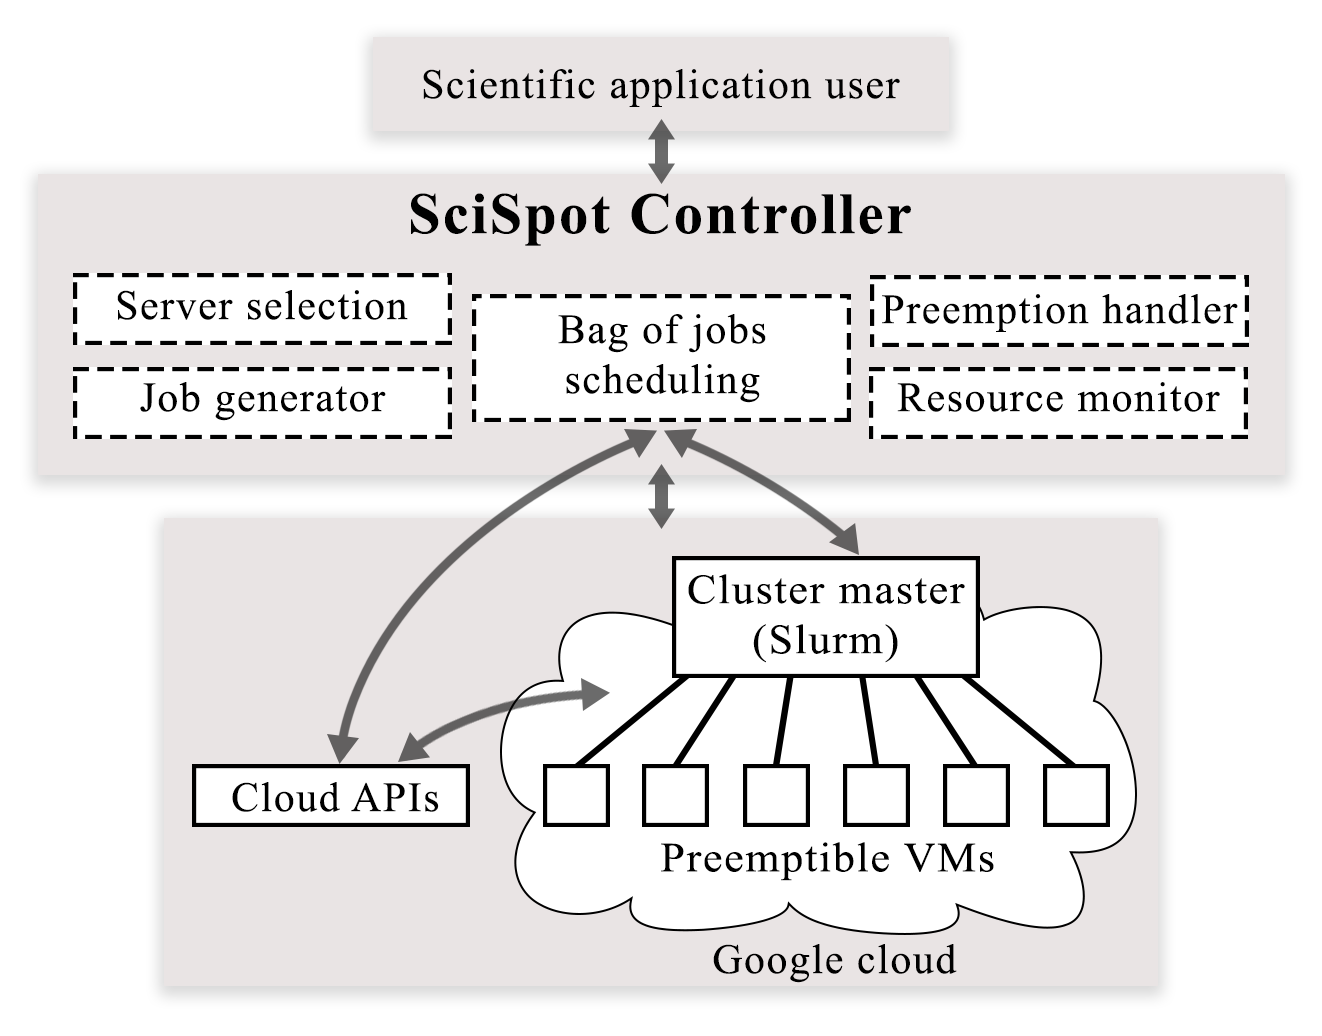
\includegraphics[width=0.3\textwidth]{../figures/Architecture.png}
\vspace*{\myfigspace}
  \caption{SciSpot architecture and system components.}
  \label{fig:arch}
  \vspace*{\myfigspace}
\end{figure}


\noindent \textbf{High-level workflow:} When a user wishes to run a bag of jobs, \sysname handles the provisioning of a cluster of transient cloud servers.
In addition, \sysname deals with the scheduling and monitoring of the bag of jobs, and with VM preemptions. 
Execution of a bag of jobs proceeds in two phases.
In the first phase, \sysname selects the ``right'' cluster configuration for a given application through a cost-minimizing exploration-based search policy, described in Section~\ref{subsec:server-selection}. 
In the second phase, \sysname proceeds to run the remaining jobs in the bag on the optimal cluster configuration. 

\prat{End design}


\sysname is implemented as a light-weight, extensible framework that makes it convenient and cheap to run scientific computing applications in the cloud.
We have implemented the \sysname prototype in Python in about 2,000 lines of code, and currently support running VMs on the Google Cloud Platform~\cite{gcp}. 
%
\sysname is implemented as a centralized controller, which implements the VM selection and job scheduling policies described in Section~\ref{sec:design}. 
The controller can run on any machine (including the user's local machine, or inside a cloud VM), and exposes an HTTP API to end-users. 
Users submit bags of jobs to the controller via the HTTP API, which then launches and maintains a cluster of cloud VMs, and maintains the job queue and metadata in a local database. 
To improve usability, we automatically generate parameter combinations for a given bag size, based on a user-provided json file with ranges and constraints for each parameter. 

\sysname integrates, and interfaces with two primary services.
First, it uses the Google cloud API~\cite{gcloud-api} for launching, terminating, and monitoring VMs.
Once a cluster is launched, it then configures a cluster manager such as Slurm~\cite{slurm} or Torque~\cite{torque}, to which it submits jobs. 
\sysname uses the Slurm cluster manager, with each VM acting as a Slurm ``cloud'' node, which allows Slurm to gracefully handle VM preemptions.
The Slurm master node runs on a small, 2 CPU non-preemptible VM, which is shared by all applications and users. 
\sysname monitors job completions and failures (due to VM preemptions) through the use of Slurm call-backs, which issue HTTP requests back to the \sysname controller.

%As part of \sysname, we also provide a base VM image with Slurm and MPI integration, along with commonly used libraries and benchmarks for scientific computing. To run an application, users must provide a location to the application source code or binaries. Integrating \sysname with container-based image management tools such as Docker~\cite{docker} and Singularity~\cite{kurtzer2017singularity} is part of our ongoing work. 





%%% Local Variables:
%%% mode: latex
%%% TeX-master: "paper"
%%% End:


\vspace*{\subsecspace}
\section{Experimental Evaluation}
\label{sec:eval}

%Opening is deliberately short because we gonna be running out of space 
In this section, we present empirical and analytical evaluation of the performance and cost of \sysname under different workloads and scales. 
Our evaluation consists of empirical analysis of the different scientific computing applications, as well as model-driven simulations for analyzing and comparing \sysname behavior under different preemption and application dynamics. 

% \begin{itemize}
% \item What is performance and cost of 
% \end{itemize}

\noindent \textbf{Environment and Workloads:} All our empirical evaluation is conducted on the Google Public Cloud, and with these representative scientific computing applications: 
% open-source
%\vspace*{\tightext}
%\begin{description}
  %TODO: Need MAX two sentence descriptions

\noindent \textbf{Nanoconfinement.}
The nanoconfiment application launches molecular dynamics (MD) simulations of ions in nanoscale confinement created by material surfaces \cite{jyto,kadupitiya2017}.

\noindent \textbf{Shapes.} The Shapes application runs an MD-based optimization dynamics to predict the optimal shape of deformable, charged nanoparticles \cite{jto1,jjzo1}. 

\noindent \textbf{LULESH.} Livermore Unstructured Lagrangian Explicit Shock Hydrodynamics (LULESH) code is a popular code to for hydrodynamics simulations of continuum material models \cite{IPDPS13:LULESH,LULESH2:changes}. 
%\end{description}
%\vspace*{\tightext}

These examples are representative of typical scientific computing applications in the broad domain of physics, materials science, and chemical engineering. These three examples are implemented as parallel programs that use OpenMP and MPI parallel computing techniques. The first two are used in nanoscale materials research \cite{jso1,jso2,solis2013generating,jjzo1,jto1,jyto} and the LULESH is a widely used benchmark \cite{IPDPS13:LULESH,LULESH2:changes}. All applications are run with default parameters unless otherwise stated. 
All applications use OpenMPI, are deployed on Slurm vXXX and 64-bit Ubuntu 18.04, and run on Google Cloud VMs with x86-64 Intel Broadwell CPUs. 
%Networking? 


\vspace*{\subsecspace}
\subsection{SciSpot Performance and Cost}

%%%%%%%%%%%%%%%%%%%%%%%%%%%%%%%%%%%%%%%%%%%%%%%%%%
\subsubsection{Impact of server exploration}

As described in Section~\ref{sec:design}, applications can be deployed on multiple types of VMs in the cloud, with each VM type having a different ``size''.
In our evaluation of parallel scientific computing applications that are CPU intensive, we are primarily interested in the number of CPUs in a VM.

When an application (i.e., bag of jobs) requests a total number of CPUs to run each of its jobs, \sysname first runs its exploration phase to find the ``right'' VM for the application.
\sysname searches for the VM that minimizes the total expected cost $E[C_{(i,n_i)}]$ of running the application, and this depends on several factors such as the parallel structure of the application, the preemption probability and the associated job recomputation time, and the price of the VM.

Thus, even if the \emph{total} amount of resources (i.e., number of CPUs) per job is held constant, the total running time of an application depends on the choice of the VM type ($i$), and the associated number of VMs ($n_i$) required to meet the allocation constraint (Section~\ref{subsec:cost-model}).
%
With preemptible instances, the total running time of a job is composed of two factors: the ``base'' running time of the job without any preemptions ($T_{(i,n_i)}$), and the expected recomputation time which depends on the probability of job failure (Equation~\ref{eq:et1}). 

\begin{figure}
  \centering
  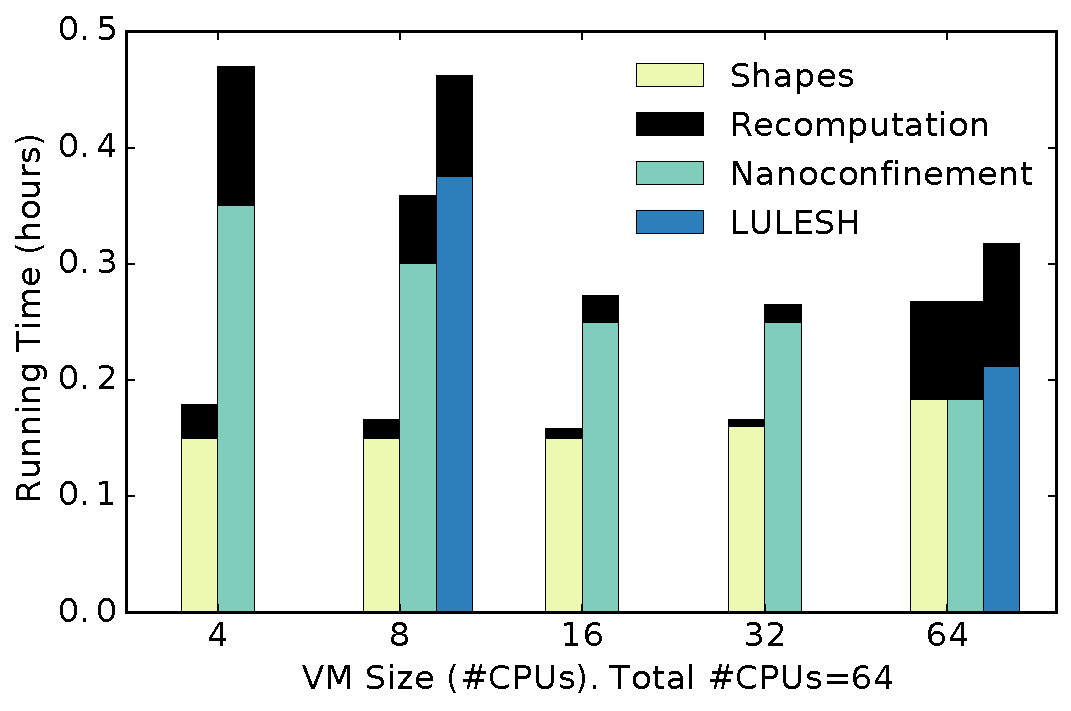
\includegraphics[width=0.4\textwidth]{../graphs/runtime-bars.pdf}
      \vspace*{\myfigspace}
  \caption{Running times of applications on different VMs. The total number of CPUs is 64, yielding different number of VMs in each case. We see different tradeoffs in the base running times and recomputation costs for the different applications.}
  \label{fig:runtimes-bar}
    \vspace*{\myfigspace}
\end{figure}


Figure~\ref{fig:runtimes-bar} shows the running times of the Nanoconfinement and Shapes application, when they are deployed on different VM sizes.
In all cases, the total number of CPUs per job is set to 64, and thus the different VM sizes yield different cluster sizes (e.g., 16 VMs with 4 CPUs or 32 VMs with 2 CPUs).


For the Nanoconfinement application, we observe that the base running times (without preemptions) reduce when moving to larger VMs, because this entails lower communication costs.
The running time on the ``best'' VM (i.e., with 32 CPUs) is nearly 40\% lower as compared to the worst case. 
On the other hand, the Shapes application can scale to a larger number of VMs without any significant communication overheads, and does not see any significant change in its running time.

Figure~\ref{fig:runtimes-bar} also shows the total expected running time $E[T_{(i,n_i)}]$, that is obtained by adding the the expected recomputation time, which depends on the expected lifetimes of the VM and the number of VMs, and is computed using the cost model introduced in Section~\ref{subsec:cost-model}. 
While selecting larger VMs may reduce communication overheads and thus improve performance, it is not an adequate policy in the case of preemptible VMs, since the preemptions can significantly increase the total running time.
We can observe this in the case of Nanoconfinement application when deployed on a 64 CPU VM---even though the base running time is lower compared to deploying the application on 2x32-CPU VMs, the recomputation time on the 64 CPU VM is almost $4\times$ higher due to the much lower expected lifetime of the larger VMs. 
Thus, on preemptible servers, there is a tradeoff between the base running time which only considers parallelization overheads, and the recomputation time.
By considering \emph{both} these factors, \sysname's server selection policy can select the best VM for an application. 


\noindent \emph{\textbf{Result:} SciSpot's server selection, by considering both the base running time and recomputation time, can improve performance by up to 40\% , and can keep the increase in running time due to recomputation to less than 5\%.}

%%%%%%%%%%%%%%%%%%%%%%%%%%%%%%%%%%%%%%%%%%%%%%%%%%
\subsubsection{Cost}

\begin{figure}
  \centering
  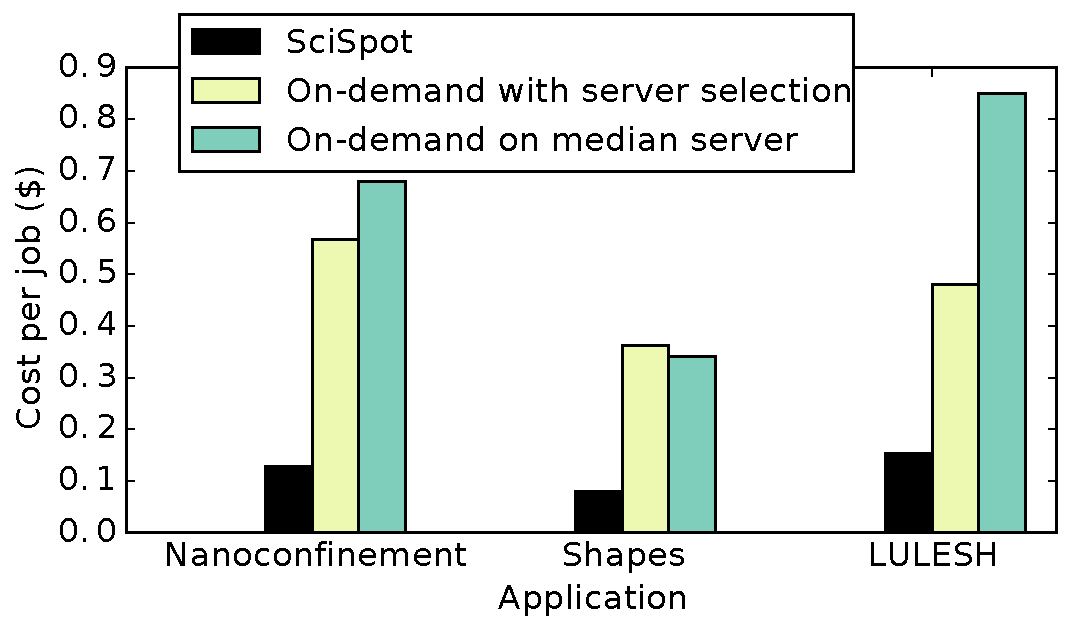
\includegraphics[width=0.4\textwidth]{../graphs/cost-only-bar.pdf}
  \vspace*{\myfigspace}
  \caption{SciSpot's use of preemptible VMs can reduce costs by up to $5\times$ compared to conventional cloud deployments.}
  \label{fig:cost-only-bar}
    \vspace*{\myfigspace}
\end{figure}


The primary motivation for using preemptible VMs is their significantly lower cost compared to conventional ``on-demand'' cloud VMs that are non-preemptible. 
Figure~\ref{fig:cost-only-bar} compares the cost of running different applications with different cloud VM deployments.
\sysname, which uses both cost-minimizing server selection, and preemptible VMs, results in significantly lower costs across the board, even when accounting for preemptions and recomputations. 
Even with \sysname's server selection, using on-demand VMs result in a $5\times$ cost increase compared to \sysname.
In the absence of server selection, we assume that the user will pick a ``median'' VM in terms of number of CPUs (in this case, 8 CPU VMs), which we also show in Figure~\ref{fig:cost-only-bar}.
Note that since \sysname's server selection considers the total turnaround time (which includes recomputation time), it may not always pick the optimal on-demand server. 

%\vj{Note that \sysname's server selection considers both the base running times and recomputation time, which may not necessarily yield the best on-demand server configuration (which only needs to be cognizant of the base running times), and thus we see that the cost for the Shapes application on the median on-demand server is slightly lower than one with \sysname's server selection. However, it is still lower than \sysname's cost. rephrase}


\noindent \emph{\textbf{Result:} SciSpot reduces computing costs by up to 5$\times$ compared to conventional on-demand cloud deployments.}

%%%%%%%%%%%%%%%%%%%%%%%%%%%%%%%%%%%%%%%%%%%%%%%%%%
\subsubsection{Comparison with HPC Overhead}

Scientific applications are typically run on large-scale HPC clusters, where different performance and cost dynamics apply.
While there are hardware differences between cloud VMs and HPC clusters that can contribute to performance differences, we are interested in the performance ``overheads''.
In the case of \sysname, the job failures and recomputations increase the total job running time, and are thus the main source of overhead.

On HPC clusters, jobs enjoy significantly lower recomputation probability, since the hardware on these clusters has MTTFs in the range of years to centuries~\cite{dongarra-ckpting}.
However, we emphasize that there exist \emph{other} sources of performance overheads in HPC clusters.
In particular, since HPC clusters have high resource utilization, they also have significant \emph{waiting} times. 
On the other hand, cloud resource utilization is low~\cite{borg} and there is usually no need to wait for resources, which is why transient servers exist in the first place. 


Thus, we compare the performance overhead due to preemptions for \sysname, and job waiting times in conventional HPC deployments.
To obtain the job waiting times in HPC clusters, we use the LANL Mustang traces published as part of the Atlas trace repository~\cite{cmu-atlas}.
We analyze the waiting time of over two million jobs submitted over a 5 year period, and compute the increase in running time of the job due to the job waiting or queuing time. 

\begin{figure}[t]
  \centering 
  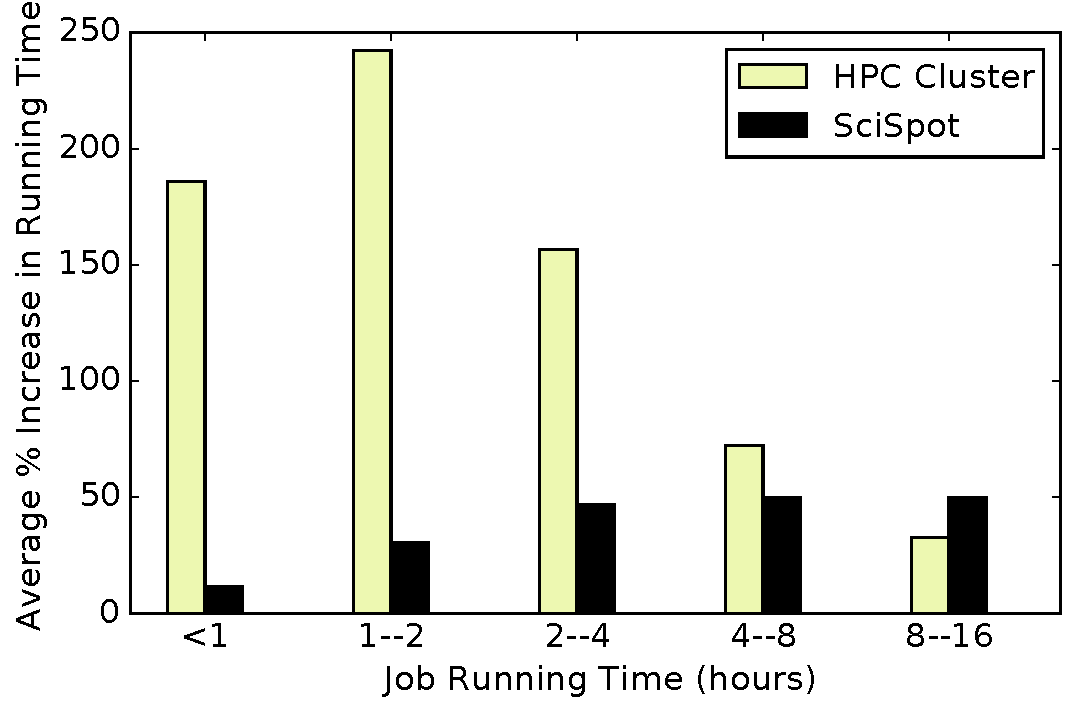
\includegraphics[width=0.4\textwidth]{../graphs/hpc-vs-scispot.pdf}
      \vspace*{\myfigspace}
  \caption{Increase in running time due to waiting/queuing on HPC clusters is significantly higher than the recomputation time for \sysname, especially for shorter jobs. }
  \label{fig:hpc-vs-scispot}
  \vspace*{\myfigspace}
\end{figure}


We define the overhead as the increase in running time which is equal to the turnaround time (i.e., the time between the job submission and successful completion) divided by the base job running time (with no waiting or premptions). 
%In HPC clusters, the overhead is the waiting time for resources, and in \sysname the overhead is the recomputation time due to preemptions.
Figure~\ref{fig:hpc-vs-scispot} compares the overhead (as percentage increase in running time) of \sysname and HPC clusters  for jobs of different lengths. We see that the average performance overhead due to waiting can be significant in the case of HPC clusters, and the job submission latency and queuing time dominate for smaller jobs, increasing their total turnaround time by more $2.5\times$.
This waiting is amortized in the case of longer running jobs, and the overhead drops off for longer jobs, to around 30\%.

On the other hand, \sysname's performance overhead is significantly smaller for jobs of up to 8 hours in length.
For longer jobs, the limited lifetime of Google Preemptible VMs (24 hours) begins to significantly increase the preemption probability and expected recomputation time.
We emphasize that these are \emph{individual} job lengths, and not the running time of entire bag of jobs.
We note that these large single jobs are rare, and for smaller jobs (within a much larger bag), both the preemption probability and recomputation overhead is much smaller. \vj{make more quantitative}

\noindent \emph{ \textbf{Result:} While preemptions can increase running times due to recomputation, this increase is small, and is between 20 to 400\% lower compared to the waiting times associated as overhead in conventional HPC clusters. }

\subsubsection{Comparison with HPC Performance}
The performance of scientific computing applications has been extensively compared on HPC and cloud setups~\cite{iosup_performance_2011, zhai_cloud_2011, marathe2013comparative, galante_analysis_2016, benedictis_cloud-aware_2014}. 
For completeness, we show the running times on the Big Red II supercomputing cluster in Table~\ref{tab:bigred2}, with 16 CPU nodes used throughout, and we see that our representative applications \emph{do not} face a penalty when deployed on the cloud. 

% This is confinement/shapes comparison against Big Red II
\begin{table}[]
  \begin{tabular}{|l|l|r|r|}
    \hline
    \# Application & Nodes & Big Red II & \sysname \\
    \hline
  	Nanoconfinement	&	1	&	2370	& 1546	\\
    Nanoconfinement	&	4	&	1140	&	851	\\
    \hline
  	Shapes	&	1	&	2649	& 1194	\\
    Shapes	&	4	&	1209	&	548	\\
    \hline
\end{tabular}
\caption{Running times (in seconds) of different applications on the Big Red II HPC cluster vs \sysname.}
\label{tab:bigred2}
  \vspace*{\myfigspace}
\end{table}




%%%%%%%%%%%%%%%%%%%%%%%%%%%%%%%%%%%%%%%%%%%%%%%%%%%%%%%%%%%%%%%%%%%%%%%%%%%%%%%%

\subsection{SciSpot Scaling}
We now turn our attention to \sysname's scaling properties. We are primarily interested in observing the behavior of running bags of jobs of different applications with different resource requirements.
In all cases unless otherwise stated, we run bags of 36 jobs, and impose that 90\% of all jobs complete (thus we target a completion of 32 jobs).
The jobs in the bags are for exploring the different parameters (i.e., doing a parameter sweep), using \sysname's automated parameter sweeping functionality described in Section~\ref{sec:impl}. For reference, the distribution of running times for the different applications is shown in Figure~\ref{fig:job-run-cdf}. 
In the rest of this section, we evaluate \sysname when the size of the cluster, the number of preemptions, and the number of jobs in the bag are increased.

\begin{figure}
  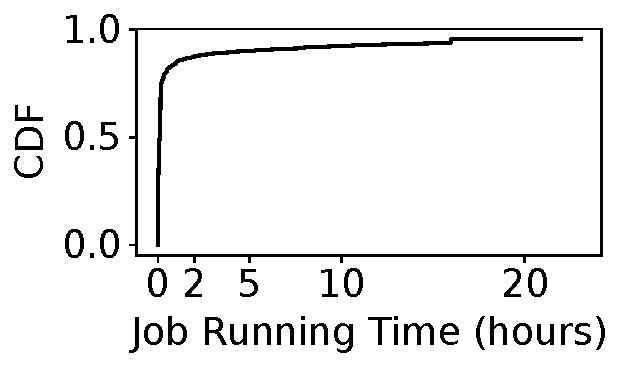
\includegraphics[width=0.2\textwidth]{../graphs/job-run-cdf.pdf}
  \vspace*{\myfigspace}
  \caption{Most HPC jobs are less than 2 hours.}
  \label{fig:job-run-cdf}
    \vspace*{\myfigspace}
\end{figure}

%%%%%%%%%%%%%%%%%%%%%%%%%%%%%%%%%%%%%%%%%%%%%%%%%%
%\vspace*{\subsecspace}
\subsubsection{Increasing Cluster Size} 

\begin{figure}
  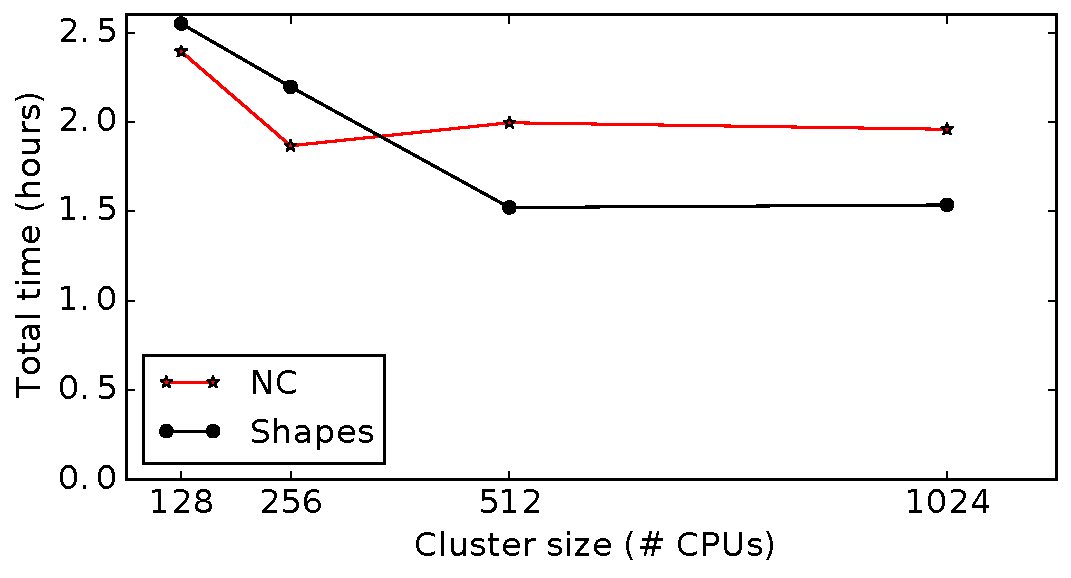
\includegraphics[width=0.4\textwidth]{../graphs/vm-per-job-scaling.pdf}
      \vspace*{\myfigspace}
  \caption{Bag of jobs running times exhibits classic parallel scaling behavior---performance improves until reaching a saturation point.}
  \label{fig:vm-per-job-scaling}
    \vspace*{\myfigspace}
\end{figure}

It is common to deploy scientific computing applications on large clusters, and we evaluate \sysname on different cluster sizes in Figure~\ref{fig:vm-per-job-scaling}.
The figure shows the total running time of the bag of jobs for the Nanoconfinement and Shapes applications as the total number of VMs (and hence total number of CPUs) increases.
For this experiment, we used \texttt{n1-highcpu-32} VMs with 32 CPUs each, and we ran four jobs in parallel on the entire cluster. 
We see classic scaling behavior: both applications can scale to a higher number of VMs up to a point, after which communication overhead starts to dominate, and the performance saturates and we see no reduction in running time. 


\begin{figure}
  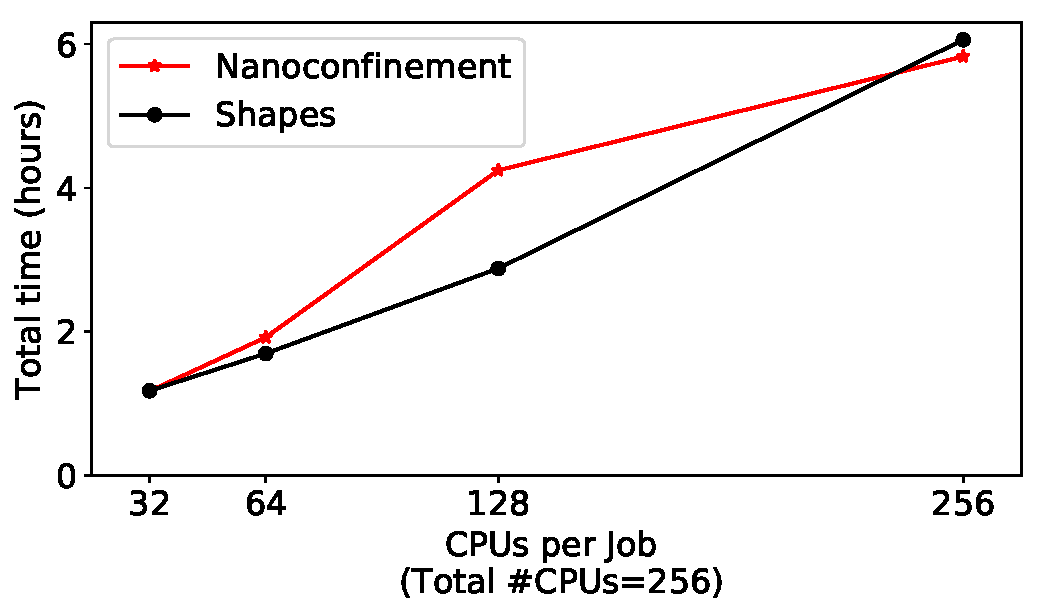
\includegraphics[width=0.2\textwidth]{../graphs/par-scaling.pdf}
      \vspace*{\myfigspace}
  \caption{\sysname can alleviate poor scaling by running more jobs in parallel and thus decreasing the intra-job parallelism (and hence number of CPUs per job, as shown in the figure).}
  \label{fig:par-scaling}
    \vspace*{\myfigspace}
\end{figure}


We note that \sysname provides the option to alleviate the parallel scaling bottleneck, by increasing the number of parallel jobs.
That is, for a given fixed cluster size, it can run more jobs in parallel, by reducing the total resources allocated and hence the parallelism 
of an individual job. 
The effect of changing the number of parallel jobs is shown in Figure~\ref{fig:par-scaling}, which shows the running time of an entire bag of jobs when the total cluster size is fixed (256 CPUs), but the number of parallel jobs and hence the number of CPUs per job changes.
We see that a \emph{smaller} number of CPUs per job limits the communication overhead, and thus reduces the total running time of the bag.
For both the NC and Shapes application, we see up to $6\times$ reduction in the total bag running time when more number of jobs are launched in parallel and a smaller number of CPUs per job are used. 


%%%%%%%%%%%%%%%%%%%%%%%%%%%%%%%%%%%%%%%%%%%%%%%%%%
\subsubsection{Increasing Bag Size}

We now evaluate \sysname's behavior when running larger bags of jobs.
Table~\ref{tab:100-jobs} shows the total running time of bags of 32 and 100 jobs.
Since \sysname reuses VMs when running jobs from a bag, it is able to take advantage of the relatively low preemption rates of VMs once they pass the first phase of early failures (Figure~\ref{fig:cdf}), and thus minimizes the number of preemptions as well as job failures. 
This makes \sysname particularly suitable for running the large bags of jobs that are required when using machine learning techniques for HPC workloads, an emerging research area in many science and engineering disciplines~\cite{ml.atomic2017,melko2017,sam2017,fu2017,long2015machine,ferguson2017machine,ward2018matminer,jcs1,jcs2,fox2019learning}, since the training and testing data needed for statistical machine learning can be generated through \sysname's bag of jobs execution model. 


%32_2_4 
\begin{table}
  \begin{tabular}{|c|r|r|r|}
    \hline
    Workload & Jobs & Time (Hours) & \# Preemptions \\
    \hline
    NC & 32  & 1.87 & 0 \\
    NC & 100  & 6.08 & 1 \\
    \hline
    Shapes & 32 & 1.47 & 0 \\
    Shapes & 100 & 4.49 & 5  \\  
    \hline
  \end{tabular}
  \caption{Running times and number of preemptions for bags of different sizes. }
  \label{tab:100-jobs}
  \vspace*{\myfigspace}
\end{table}




%%%%%%%%%%%%%%%%%%%%%%%%%%%%%%%%%%%%%%%%%%%%%%%%%%
\subsubsection{Increasing Preemptions}

By reusing VMs across a bag of jobs and taking advantage of the low preemption rates during the middle of the 24 hour life of the preemptible VMs, the \emph{expected} job failure rates and recomputation times are fairly small with \sysname (as shown in Figures~\ref{fig:runtimes-bar},~\ref{fig:hpc-vs-scispot}).
However, preemption rates can increase when the cloud operator sees high demand for resources.
Figure~\ref{fig:fails-time} shows the running time of the bag of 32 Nanoconfinement jobs on a cluster of 4 \texttt{n1-highcpu-32} VMs, when different number of VMs are preempted. 

We see that even with a high number of preemptions, the running time only increases by 50\%. 
We note that a higher than expected preemption rate (as shown in the figure) is rare, and happens with a vanishingly small likelihood. 
This shows that \sysname is robust and can provide acceptable performance even under extreme, adverse conditions. 

\begin{figure}[t]
  \centering 
  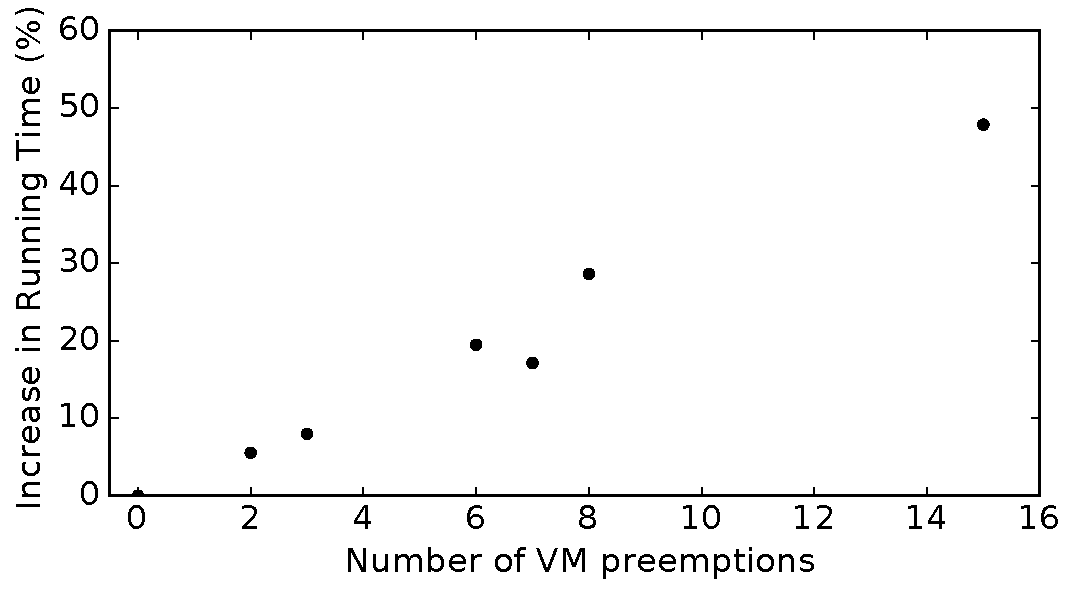
\includegraphics[width=0.4\textwidth]{../graphs/confin-fails-vs-time-relative.pdf}
      \vspace*{\myfigspace}
  \caption{The increase in running time due to preemptions is under 50\%, even when the number of preemptions is high.}
  \label{fig:fails-time}
\end{figure}


%Summary of results? 

%%%%%%%%%%%%%%%%%%%%%%%%%%%%%%%%%%%%%%%%%%%%%%%%%%


% \begin{figure}
%   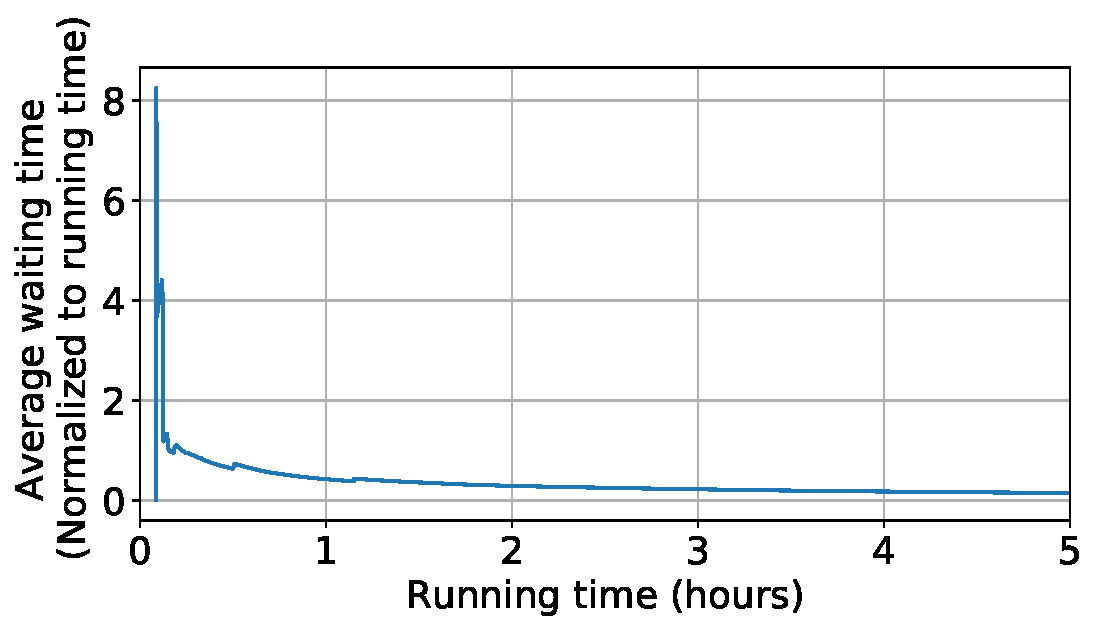
\includegraphics[width=0.4\textwidth]{../data/waiting_cumul.pdf}
%   \caption{The average waiting time (normalized to running time) of jobs of different length.}
%   \label{fig:hpc-wait-cdf}
% \end{figure}



%%% Local Variables:
%%% mode: latex
%%% TeX-master: "paper"
%%% End:


\vspace*{\subsecspace}
\section{Related Work}
\label{sec:related}


\sysname builds upon a large body of prior work on running scientific computing applications on the cloud, and the various facets of transient cloud computing.  

\vspace*{\subsecspace}
\subsection{Cloud Computing For Science}
Running scientific applications on the cloud introduces many tradeoffs compared to conventional HPC clusters, along the dimensions of performance, cost, scalability, convenience, and reproducability.
These tradeoffs are explored in~\cite{iosup_performance_2011, zhai_cloud_2011, marathe2013comparative, galante_analysis_2016, benedictis_cloud-aware_2014}.
In general, clouds can provide increased elasticity, lower waiting times, and more choices in resource allocation that can be tailored to the application.
The cloud resource model is also present in platforms like nanoHUB~\cite{nanohub}, that provide easy execution and dissemination of nanotechnology simulation applications.
%such as Ref.~\cite{kadupitiya2017}.
Outside of the bags of jobs execution model, price optimizations for scientific workflows in the cloud is discussed in~\cite{gari_learning_2019}. 
While bags of tasks~\cite{varshney_autobot_2019} are often used for parallel applications, \sysname is the first to use the bags of \emph{jobs} abstraction for efficient and effective use of transient servers. 

%\subsubsection{Bags of Jobs}
\vspace*{\subsecspace}
\subsection{Transient Cloud Computing}

%The low cost of transient cloud servers has made them very appealing, inspite of their preemptible nature, and their efficient and effective use has been a significant amount of research~\cite{prateek-thesis}. 
The challenges posed by Amazon EC2 spot instances, the first transient cloud servers, have received significant attention from both academia  and industry~\cite{spotinst}. 
Since spot instances are significantly cheaper than the equivalent on-demand servers, they are attractive for running preemption and delay tolerant batch jobs~\cite{spoton, jain14demand, yi2010reducing, conductor, liu-spot, spot-run, dubois2016optispot}.
A crucial component of EC2 spot instances is their dynamic auction-based pricing, and choosing the ``right'' bid price to minimize cost and performance degradation is the focus of much of the past work on transient computing~\cite{bidding4,mihailescu2012impact,bidding7,bidding1,bidding8,bidding3,bidding6,bid-cloud,bidding5,wolski_probabilistic_2017, guo_bidding_2015}.
However, as explained in Section~\ref{subsec:need-for-empirical}, it remains to be seen how Amazon's recent change~\cite{bid-change} in the preemption model of spot instances affects prior work.


On the other hand, the effective use of transient resources provided by other cloud providers such as Google, Microsoft, Packet, and Alibaba largely remains unexplored. 
Ours is the first work that studies the preemption characteristics and addresses the challenges involved in running large-scale applications on the Google Preemptible VMs, and provides insights on the unique preemption dynamics, as explained in Section~\ref{sec:preemption-dynamics}.

\vspace*{\subsecspace}
\subsubsection{Preemption Mitigation}
Effective use of transient servers usually entails the use of fault-tolerance techniques such as checkpointing~\cite{flint}, migration~\cite{spotcheck}, and replication.
In the context of HPC workloads,~\cite{marathe2014exploiting,gong_monetary_2015,xiang_spotmpi:_2011} develop checkpointing and bidding strategies for MPI applications running on EC2 spot instances, based on older spot pricing models. 
%, which are inherently memoryless and not applicable in our case. 
Periodic checkpointing~\cite{dongarra_fault_nodate} is not appropriate in our case because preemptions are not memoryless. 

By treating bags of jobs as an execution unit, allowing some jobs to fail, and using insights from preemption models, we show that it is possible to reduce the recomputation times to acceptable levels even without the  use of periodic  checkpointing that imposes additional deployment and performance overheads. 
%The first step towards mitigating preemptions is understanding their characteristics. 
Our preemption model for Google preemptible VMs developed in Section~\ref{sec:preemption-dynamics} provides a novel characterization of bathtub shaped failure rates not captured by the classic Weibull distribution, and is distinct from prior efforts~\cite{mudholkar1993exponentiated, crevecoeur1993model}. 

%extends the classic Weibull-distribution based bathtub models~\cite{mudholkar1993exponentiated, crevecoeur1993model} by introducing exponential reclamation near the deadline and additional paramters that capture and explain the preemption dynamics. 

\vspace*{\subsecspace}
\subsubsection{Server Selection}

Optimized server selection is an important problem in cloud computing, and especially for transient servers because of the cost-performance-preemption tradeoff involved. 
Similar to \sysname, SpotOn~\cite{spoton} is also a batch computing service that selects servers based on job characteristics and failure rates of different EC2 spot VMs. However, it is restricted to individual, single-VM batch jobs, and its design is tied to EC2 spot instances.
The state of the art transient server selection involves the use of multiple types of VMs~\cite{exosphere}, and selecting a heterogeneous cluster can reduce the likelihood of mass concurrent preemptions.
However, since scientific computing applications are mostly synchronous, even a single failure affects the entire job, and heterogeneous clusters are not required, and are in fact, detrimental~\cite{exosphere}. 
Server selection is important even outside of preemptible VMs---developing bayesian optimization and application performance model based search for the ``best'' cloud VM is an active research area~\cite{alipourfard_cherrypick, yadwadkar_selecting_2017}, but these techniques do not  account  for preemptions. 

\begin{figure}[t]
  \centering 
       \vspace*{\myfigspace} 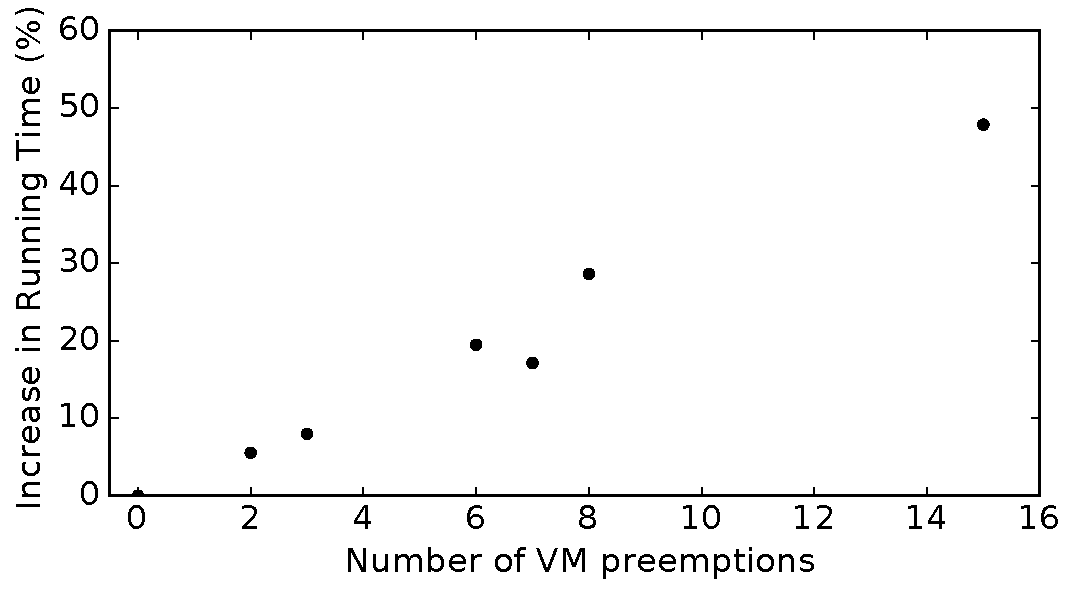
\includegraphics[width=0.22\textwidth]{../graphs/confin-fails-vs-time-relative.pdf}
      \vspace*{\myfigspace}
  \caption{The increase in running time due to preemptions is under 50\%, even when the number of preemptions is high.}
  \label{fig:fails-time}
        \vspace*{\myfigspace}
\end{figure}




\vspace*{\subsecspace}
%Parameter sweep aka bags of jobs ~\cite{casanova_heuristics_2000}

%But nothing for bags of jobs themselves.. 


% \subsubsection{Fault-tolerance}

% All the past work was on EC2 spot market with gang failures and independent markets~\cite{marathe2014exploiting, gong_monetary_2015}.
% However this assumption has now changed, and failures can happen anytime.
% Our failure model is more general, and applies to both cases.



% \cite{dongarra_fault_nodate} has a discussion of checkpointing frequency which is comprehensive. Replication is another way~\cite{walters_replication-based_2009}

% Non periodic checkpointing~\cite{bougeret_checkpointing_2011}


% \subsubsection{Failure Modeling}



% Crevecour etc. 



% \subsubsection{Server Selection}
% Exploring a large configuration space using bayesian optimization methods in CherryPick~\cite{alipourfard_cherrypick} and Metis~\cite{li2018metis}.

% Can also use Latin Hypercube sampling for parameter exploration?




%%% Local Variables:
%%% mode: latex
%%% TeX-master: "paper"
%%% End:


%% 10 pages plus references 

{
\bibliographystyle{acm}
\interlinepenalty=10000 %%%%For fixing url-related errors only 
\bibliography{scicloud}
}


\end{document}


%%% Local Variables:
%%% mode: latex
%%% TeX-master: t
%%% End:
